% =============================================================================
% ChaoticNet 物理竞赛论文 主文件
% 截稿：2026-09-15
% 编译：xelatex main.tex（中文需 xelatex，不要用 pdflatex）
% =============================================================================

\documentclass[a4paper,12pt]{ctexart}   % 正文小四（12pt），竞赛格式规范

% --- 数学 ---
\usepackage{amsmath, amssymb, amsthm}
\usepackage{bm}                                    % 粗体数学符号
\usepackage{physics}                               % \dv \pdv \abs 等

% --- 排版 ---
\usepackage[margin=2.5cm]{geometry}
\usepackage{setspace}
\setstretch{1.655}                       % 行距≈24磅（12pt 正文 baselineskip 14.5pt ×1.655）
\emergencystretch=3em                    % 小四下容差，消除不可断 \texttt/公式行的溢出
\usepackage{titlesec}
\usepackage{enumitem}

% --- 图表 ---
\usepackage{graphicx}
\graphicspath{{figures/}{../data/figures/}{../data/sim/figures/}{../data/real_validation/figures/}%
              {../data/v2_50trial_2026-06-11/}%
              {../data/sim/figures/v1_baseline_2026-06-11/}%
              {../data/rc/figures/v1_baseline_2026-06-11/}%
              {../data/pinn/figures/v1_baseline_2026-06-11/}}
\usepackage{booktabs}
\usepackage{caption}
\usepackage{float}
\usepackage{subcaption}

% --- 算法 / 代码 ---
\usepackage{algorithm}
\usepackage{algpseudocode}
\usepackage{listings}
\lstset{basicstyle=\ttfamily\small, breaklines=true, frame=single}

% --- 引用 ---
\usepackage[colorlinks=true, linkcolor=blue, citecolor=blue, urlcolor=blue]{hyperref}
\usepackage{cleveref}

% --- 文献 ---
% 参考文献采用 GB/T 7714—2015 顺序编码制；样式文件随项目放在 texstyles/gb7714/。
\usepackage[backend=biber, style=gb7714-2015, sorting=none]{biblatex}
\addbibresource{references.bib}
\let\cite\supercite   % 正文文献引用统一改为右上标数字

% --- 目录样式：章节页码统一为正常字号、不加粗（与子节一致；标题保留加粗以示层级）---
\makeatletter
\AtBeginDocument{%
  \renewcommand*\l@section[2]{%
    \ifnum \c@tocdepth >\z@
      \addpenalty\@secpenalty
      \addvspace{1.0em \@plus\p@}%
      \setlength\@tempdima{1.5em}%
      \begingroup
        \parindent \z@ \rightskip \@pnumwidth
        \parfillskip -\@pnumwidth
        \leavevmode \bfseries
        \advance\leftskip\@tempdima
        \hskip -\leftskip
        #1\nobreak\hfil
        \nobreak\hb@xt@\@pnumwidth{\hss \normalfont\mdseries #2%
                                   \kern-\p@\kern\p@}\par
      \endgroup
    \fi}%
}
\makeatother

% --- 自定义命令 ---
\newcommand{\tauL}{\tau_{\mathrm{L}}}              % Lyapunov 时间
\newcommand{\thetaone}{\theta_1}
\newcommand{\thetatwo}{\theta_2}

% --- 交叉引用中文名（cleveref 默认输出 section/figure/table，统一改为中文）---
\crefname{section}{节}{节}
\Crefname{section}{节}{节}
\crefname{subsection}{节}{节}
\Crefname{subsection}{节}{节}
\crefname{figure}{图}{图}
\Crefname{figure}{图}{图}
\crefname{table}{表}{表}
\Crefname{table}{表}{表}
\crefname{equation}{式}{式}
\Crefname{equation}{式}{式}
\crefname{algorithm}{算法}{算法}
\Crefname{algorithm}{算法}{算法}
\crefname{appendix}{附录}{附录}
\Crefname{appendix}{附录}{附录}

% --- 图表标题：比正文小一号 + 标签加粗，与正文区分 ---
\captionsetup{font={small,bf}}

% --- 正文强调不切换字形或字号，避免与普通正文产生视觉尺寸差异 ---
\renewcommand{\emph}[1]{#1}

% =============================================================================
\title{物理约束神经网络在双摆混沌预测中的应用\\
       \large 本科实验室级精度下的可信预测窗口扩展}
\author{}
\date{}

\begin{document}
\maketitle
\pagestyle{plain}   % 页码居中置于页脚，去除每页左上角的章节名页眉

% =============================================================================
\begin{abstract}
{\setlength{\parindent}{0pt}\setlength{\parskip}{0.8em}\setstretch{1.42}
双摆是经典的低维确定性混沌系统，其轨迹对初值极度敏感；传统观点认为，可信预测窗口通常不超过约一个 Lyapunov 时间（相邻轨迹偏离的特征时间）。本研究以双摆动力学为测试平台，把物理先验按由无到有、由弱到强分为四档，定量评估其在闭环递推预测任务中的表现：纯数据驱动的回声状态网络（Echo State Network, ESN）与多层感知机（multilayer perceptron, MLP）不含任何物理先验，物理约束神经网络（Physics-Informed Neural Network, PINN）以拉格朗日力学残差作为损失项弱约束，混合模型（Hybrid）则直接以解析运动方程为主干、仅用网络学习残差。所用数据来自本科实验室级硬件平台：双摆经手动释放，以 60\,fps 手机相机视觉追踪；初始角度与角速度由视觉追踪的轨迹反演获得，其中初始角度的估计不确定度约为 $0.5^\circ$。

在 50 组随机初值的仿真统计中（每个模型独立训练多次，取逐次运行中位数以反映训练随机性），
以物理结构由弱到强排列的三个模型，其中位可信预测视界（以角度欧氏偏差超过 $10^\circ$ 为阈值）
均超过纯数据驱动的 ESN 基线（0.70\,s，约 $0.91$ 个 Lyapunov 时间 $\tauL$，与文献给出的储池计算基线相符）：
解析先验最完整的混合模型（Hybrid）达 2.85\,s（$3.74\,\tauL$，约 4.1 倍），纯数据多层感知机（MLP）达 1.55\,s（$2.03\,\tauL$，2.2 倍），
带拉格朗日物理损失的 PINN 达 0.88\,s（$1.15\,\tauL$，1.3 倍）。更关键的是，在 29 段真实双摆视频上的零样本仿真到真实（sim$\to$real）迁移中，
物理先验模型仍显著占优——Hybrid 与 PINN 中位视界约为 ESN（0.167\,s）的 $2.5\text{--}2.7$ 倍。
物理损失恰在分布迁移下才显现价值：相同训练设置下，带物理损失（$\lambda_{\mathrm{phys}}=0.1$）
相对纯数据（$\lambda_{\mathrm{phys}}=0$）将真实中位视界由 0.36\,s 提升至 0.42\,s（约 $1.16\times$），
而这一增益在仿真内部并不出现（干净仿真数据上纯数据拟合反而更准）。我们进一步发现，sim$\to$real 迁移质量的首要决定因素是仿真保真度：采用与真实硬件一致的\emph{分布质量}摆模型，迁移质量显著优于理想点质量模型。为回答真实视界为何短于仿真内部值，我们用同口径的解析积分器隔离单一误差源，构造三条“天花板”作定量分解：实测视界 $0.42$\,s 远低于纯阻尼失配天花板（$1.35$\,s）与纯初值不确定天花板（$1.90$\,s），说明 $4$\,s 短窗内主导因素是模型逼近误差与初值估计误差的组合，而非无摩擦模型的阻尼失配——“修阻尼”在此无收益，提升初值测量精度才是方向。

高保真物理建模与物理约束可显著延长混沌预测窗口；物理损失在 sim$\to$real 迁移中尤具价值，
为低成本实验中的机器学习辅助动力学预测提供了可行路径。

\textbf{关键词：} 双摆；混沌；物理约束神经网络；回声状态网络；Lyapunov 时间
\par}
\end{abstract}

\begin{abstract}
{\setlength{\parindent}{0pt}\setlength{\parskip}{0.8em}
\textbf{Abstract.} The double pendulum is a classical low-dimensional
deterministic chaotic system. Conventional wisdom holds that trajectories can be reliably
predicted only within roughly one Lyapunov time.

We compare a purely data-driven Echo State Network (ESN)
against a Physics-Informed Neural Network (PINN) constrained by the Lagrangian equations of
motion, on closed-loop prediction of double-pendulum trajectories. All training data are
designed to match an undergraduate-lab-grade hardware platform:
manual pendulum release, a 60\,fps consumer-phone camera, and initial states recovered from
video tracking (estimation uncertainty $\approx 0.5^\circ$). We further implement a Hybrid (Universal-Differential-Equation
style) model fusing the analytical right-hand side with a small residual network, and report
results on both undamped and damped (fitted joint damping, $b \approx 1.66\times10^{-5}$\,N$\cdot$m$\cdot$s/rad) ground truth.

Across 50 random initial conditions, with each model trained
independently multiple times (reporting the median of per-run medians to reflect training
stochasticity), models carrying stronger physical structure outperform the data-driven ESN
(median horizon $0.70$\,s on chaotic trials, $10^\circ$ threshold): the fully-analytic-prior
Hybrid reaches $2.85$\,s ($\approx 4.1\times$), a pure-data MLP $1.55$\,s ($2.2\times$), and the
Lagrangian-physics-loss PINN $0.88$\,s ($1.3\times$). Normalized by the self-measured Lyapunov
time $\tauL = 0.76$\,s, these are $0.91/1.15/2.03/3.74\,\tauL$ for ESN/PINN/MLP/Hybrid, placing
our ESN baseline in line with the one-to-two Lyapunov times reported for reservoir computing.
Crucially, on 29 real double-pendulum videos under zero-shot sim$\to$real transfer,
physics-prior models retain a clear advantage (Hybrid and PINN median horizon
$\approx 2.5\text{--}2.7\times$ that of ESN, $0.167$\,s). The physics loss proves its worth
precisely under distribution shift: with identical training, $\lambda_{\mathrm{phys}}=0.1$
raises the real median horizon from $0.36$\,s ($\lambda_{\mathrm{phys}}=0$) to $0.42$\,s
($\approx 1.16\times$), a gain absent in-simulation, where clean-data fitting is most accurate.
We further find the dominant driver of sim$\to$real transfer is simulation fidelity: a
distributed-mass pendulum model matching the real hardware transfers markedly better than an
idealized point-mass model. A three-ceiling error decomposition shows the short real horizon is
governed primarily by the model's own approximation error, together with measurement noise and
initial-state uncertainty, rather than by the undamped model's damping mismatch.

High-fidelity physical modeling together with physics-informed
constraints substantially extend the trustworthy prediction window for chaotic systems in
low-cost experimental conditions, with the physics loss's value emerging precisely under
sim$\to$real distribution shift, providing a feasible pathway for ML-assisted dynamics
prediction on undergraduate-lab-grade hardware.

\textbf{Keywords:} double pendulum; chaos; physics-informed neural network;
echo state network; Lyapunov time
\par}
\end{abstract}

% =============================================================================
\newpage
{\hypersetup{linkcolor=black}\tableofcontents}
\newpage

% =============================================================================
\section{引言}
\label{sec:intro}

\subsection{研究背景}

混沌系统预测兼具理论深度与工程价值。大气是典型的高维混沌系统，数据驱动的天气预报模型 GraphCast 与盘古气象已在多数指标上超越传统数值预报系统，并能在分钟级时间内完成十天预报 \cite{lam2023graphcast,bi2023pangu}；而将物理定律作为先验约束嵌入学习模型的范式，也已在更广的工程与环境系统中得到系统性梳理 \cite{willard2022integrating}。

\paragraph{双摆混沌动力学}
双摆系统在 18 世纪被 Lagrange 系统研究，是最简单的能够呈现确定性混沌的二自由度
力学系统。Shinbrot 等人用照相法首次在实验上验证了双摆轨迹的
正 Lyapunov 指数特性 \cite{shinbrot1992}，Levien 与 Tan 设计了适用于
本科教学的双摆装置以演示其对初值的敏感依赖 \cite{levien1993pendulum}，Stachowiak 与 Okada
用谱方法系统刻画了相空间中混沌区与准周期区的边界 \cite{stachowiak2006chaotic}。Vitanov 等
计算了双摆在不同能量层级下的最大 Lyapunov 指数 $\lambda_{\max}$，
给出 Lyapunov 时间 $\tauL = 1 / \lambda_{\max}$ 的解析估算 \cite{vitanov2010lyapunov}。
混沌系统之所以难以长时间预测，根源在于初值的指数敏感性：
两条邻近轨迹的状态距离按 $e^{t / \tauL}$ 放大，无论初值精度多高，
可信预测都被限制在约 $1$ 个 Lyapunov 时间之内，这是混沌动力学的经典结论 \cite{ott2002}。

\paragraph{数据驱动预测：储池计算}
Echo State Network（ESN）由 Jaeger 与 Haas 提出，用稀疏随机
循环网络的“储池”提取高维非线性特征，仅训练线性读出层 \cite{jaeger2004}。
Lu 等与 Pathak 等系统研究了 ESN
在 Lorenz、Kuramoto-Sivashinsky 等混沌系统上的预测能力，给出“约 $1$--$2$ 个
Lyapunov 时间”的视界基线 \cite{lu2017reservoir,pathak2018}。ESN 不利用任何物理先验，纯靠时间序列学习。

\paragraph{物理约束与混合建模}
Raissi 等提出 Physics-Informed Neural Network（PINN），
将偏微分方程（partial differential equation, PDE）残差作为正则化项嵌入训练损失，使神经网络在求解 PDE 时遵守物理约束 \cite{raissi2019}。
针对哈密顿系统与拉格朗日系统，Greydanus 等提出 Hamiltonian
Neural Network（哈密顿神经网络，HNN）\cite{greydanus2019}，Cranmer 等提出 Lagrangian Neural
Network（拉格朗日神经网络，LNN）\cite{cranmer2020}；这两类模型通过学习系统的能量函数，在结构上保持能量守恒。
Karniadakis 等在 \textit{Nature Reviews Physics}
综述了该领域 \cite{karniadakis2021review}。
Chen 等提出的 Neural ODE（神经常微分方程）将动力学学习视为
连续时间常微分方程的求解 \cite{chen2018neuralode}，
Rackauckas 等进一步把已知物理方程与神经网络结合
为 Universal Differential Equation（通用微分方程，UDE）\cite{rackauckas2020universal}，即本文所称的 \emph{解析-NN 混合}范式。

\paragraph{本研究定位}
现有文献大多在数值仿真层面对比这些方法，鲜有在低成本实物装置（本科实验室级硬件、
手动释放、手机相机视觉测量与初值反演）下做端到端的可预测窗口量化。
本文聚焦这一空缺，并开源全套可复现材料：硬件加工图与物料清单（bill of materials, BOM）、
全部软件，以及 29 段真实轨迹的分析窗数据集与由原始录像重建逐帧结果的脚本
（详 \cref{sec:apparatus} 与 \cref{sec:appendix-reproducibility}）。
更重要的是，双摆在本文中被用作一个可\emph{精确开关物理先验}的最小试验台：在同一套数据与评测口径下，
把物理约束从无（纯数据 MLP）、到弱（物理损失 PINN）、再到强（解析先验 Hybrid）逐级注入，
使我们得以在受控条件下诚实回答\emph{物理约束何时有用、增益有多大}，而非停留在单一模型的点对比。

\subsection{研究问题}
\textbf{核心问题：} 在本科实验室级的测量精度下（相机 60\,fps、
初值状态估计不确定度约 $0.5^\circ$），为神经网络引入物理约束，能否显著延长它对混沌轨迹的可信预测窗口？

\subsection{本文贡献}
\begin{enumerate}[leftmargin=2em]
  \item 设计并实现了一套总成本约 580\,元的双摆实验装置（详 \cref{sec:apparatus}），
        设计目标为摆轴衰减时间常数 $\tau \geq 30$\,s，实测达 $\tau \approx 130$\,s（约 $4\times$ 目标，见 \cref{sec:apparatus}），以提供 AI 训练所需的“干净”混沌窗口；
  \item 对比 ESN、纯数据 MLP、PINN（拉格朗日物理损失）与 Hybrid（解析先验$+$残差）四类模型，
        在相同训练 / 预测设置、多次独立训练下量化物理结构的贡献；
  \item 揭示 sim$\to$real 零样本迁移的两个关键：仿真保真度（与真实硬件一致的\emph{分布质量}建模）
        为首要驱动，物理损失作为分布迁移下的稳健性正则提供二阶增益（在同分布仿真内反而无益）；
  \item 在初值不确定度上进行敏感性扫描（\cref{sec:results-sensitivity}），
        以解析真解为纯净参照，分离出混沌放大与模型逼近误差各自的贡献，
        并给出约 $\pm 0.5^\circ$ 初值不确定度下本研究结论的退化幅度。
\end{enumerate}

\subsection{论文结构}
\cref{sec:physics-model} 给出双摆拉格朗日动力学；\cref{sec:simulation} 介绍数值基线；
\cref{sec:apparatus} 描述硬件平台；\cref{sec:vision} 给出视觉追踪管线；
\cref{sec:ai-models} 介绍 ESN、Hybrid 与 PINN 三类模型；\cref{sec:results} 给出仿真内的对比结果与初值敏感性扫描；
\cref{sec:sim2real} 是本文的核心部分，报告 29 段真实轨迹上的零样本 sim$\to$real 迁移、
物理损失的价值边界，以及真实短视界的三天花板误差分解；\cref{sec:discussion} 讨论局限与展望；
\cref{sec:conclusion} 归纳结论。
附录中，\cref{sec:appendix-reproducibility} 给出完整的复现入口与目录结构，
\cref{sec:appendix-hyperparams} 列出各模型关键超参数，\cref{sec:appendix-ablation} 报告消融实验，
\cref{sec:appendix-honesty} 记录方法论上的自我修正。

% =============================================================================
\section{物理模型}
\label{sec:physics-model}

\subsection{拉格朗日方程}
双摆是非线性振动理论中的经典强耦合系统 \cite{nayfeh2008nonlinear}。
本研究的实物为\emph{分布质量}物理摆 \cite{rafat2009distmass}：上下摆杆是质量沿杆身分布的刚性铝臂，下摆末端另加配重，
质量并非集中于杆末端的理想质点。故以各摆的总质量 $M_i$、质心到其转轴的距离 $L_{c,i}$，
以及绕转轴的转动惯量建模——上摆绕固定顶轴 $O$ 的转动惯量记 $I_1^{O}$，
下摆绕关节轴 $A$ 的转动惯量记 $I_2^{A}$。设关节间距（顶轴到关节）为 $L_1$，
下摆几何长度为 $L_2$，两摆杆与竖直方向夹角分别为 $\thetaone, \thetatwo$（\cref{fig:pendulum-schematic}）。

\begin{figure}[htbp]
\centering

\includegraphics[width=0.5\linewidth]{fig_pendulum_schematic.png}
\caption{双摆物理模型示意图。两摆杆按分布质量刚体建模：$M_1, M_2$ 为各摆总质量，$L_{c1}, L_{c2}$ 为质心到相应转轴的距离，$L_1, L_2$ 为几何长度，$\thetaone, \thetatwo$ 为两摆与竖直方向的夹角，$g$ 为重力加速度。}
\label{fig:pendulum-schematic}
\end{figure}

拉格朗日量
\begin{equation}
\mathcal{L} = T - V
\label{eq:lagrangian}
\end{equation}
其中动能与势能为（下摆动能已用平行轴定理 $I_2^{A} = I_2^{\mathrm{cm}} + M_2 L_{c2}^2$ 合并）
\begin{align}
T &= \tfrac{1}{2}\left(I_1^{O} + M_2 L_1^2\right) \dot{\thetaone}^2
   + M_2 L_1 L_{c2} \cos(\thetaone - \thetatwo)\, \dot{\thetaone}\dot{\thetatwo}
   + \tfrac{1}{2} I_2^{A} \dot{\thetatwo}^2 \\
V &= -\left(M_1 L_{c1} + M_2 L_1\right) g \cos\thetaone - M_2 L_{c2}\, g \cos\thetatwo
\end{align}

\noindent 应用 Euler--Lagrange 方程
\[
\frac{d}{dt}\frac{\partial \mathcal{L}}{\partial \dot{\theta}_i}
- \frac{\partial \mathcal{L}}{\partial \theta_i} = 0
\]
得到运动方程的矩阵形式
\begin{equation}
\bm{M}(\bm{\theta}) \, \ddot{\bm{\theta}} = \bm{b}(\bm{\theta}, \dot{\bm{\theta}})
\label{eq:eom}
\end{equation}
其中质量矩阵与力向量为
\begin{align}
\bm{M}(\bm{\theta}) &= \begin{pmatrix}
  I_1^{O} + M_2 L_1^2 & M_2 L_1 L_{c2} \cos(\thetaone - \thetatwo) \\
  M_2 L_1 L_{c2} \cos(\thetaone - \thetatwo) & I_2^{A}
\end{pmatrix} \\
\bm{b}(\bm{\theta}, \dot{\bm{\theta}}) &= \begin{pmatrix}
  -M_2 L_1 L_{c2} \sin(\thetaone - \thetatwo) \dot{\thetatwo}^2 - (M_1 L_{c1} + M_2 L_1) g \sin\thetaone \\
   M_2 L_1 L_{c2} \sin(\thetaone - \thetatwo) \dot{\thetaone}^2 - M_2 L_{c2}\, g \sin\thetatwo
\end{pmatrix}
\end{align}
质量集中于杆末端的理想点质量摆是本式的特例
（$L_{c1}=L_1,\ L_{c2}=L_2,\ I_1^{O}=M_1 L_1^2,\ I_2^{A}=M_2 L_2^2$）。
本研究按实测物料清单（BOM，见 \texttt{diagrams/parts/BOM.md}）反推分布质量参数：
$L_1 = 250$\,mm, $L_2 = 200$\,mm，总质量 $M_1 \approx 96.5$\,g, $M_2 \approx 139$\,g，
质心距 $L_{c1} \approx 122$\,mm, $L_{c2} \approx 145$\,mm，转动惯量
$I_1^{O} \approx 1.99\times 10^{-3}\,\mathrm{kg\,m^2}$,
$I_2^{A} \approx 3.54\times 10^{-3}\,\mathrm{kg\,m^2}$，$g = 9.81$\,m/s$^2$。
采用与真实硬件一致的分布质量模型，是后文 sim$\to$real 零样本迁移得以成立的关键（见 \cref{sec:sim2real-decomp}）。
具体实现见 \texttt{sim/baseline.py}，符号求逆得到 $\ddot{\bm{\theta}} = \bm{M}^{-1} \bm{b}$。

\subsection{混沌特征：最大 Lyapunov 指数实测}
我们对 50 组随机初值（$\thetaone, \thetatwo \in [-90^\circ, 90^\circ]$ 均匀采样，
$\omega = 0$ 静止释放）实施基于轨迹分叉的最大 Lyapunov 指数估算：对每组参考初值
施加 $\varepsilon = 10^{-6}$\,rad 扰动，跟踪两条由 RK45（四/五阶 Runge--Kutta 自适应步长法）积分得到的轨迹之间的 4 维相空间欧氏距离
$d(t)$ 在 $3$\,s 内的指数增长，对数线性区拟合得到斜率 $\lambda_{\max}$。
50 组随机初值中 48 组有效拟合（另 2 组分叉斜率非正剔除）的分布（分布质量模型）：均值 $\bar\lambda_{\max} = 1.21$\,s$^{-1}$（$1/\bar\lambda_{\max} = 0.83$\,s），
中位 $\lambda_{\max}^{\mathrm{med}} = 1.31$\,s$^{-1}$（$\tauL^{\mathrm{med}} = 0.76$\,s）。
\emph{方法学注：} 此处 $\tauL = 0.76$\,s 取自分叉曲线 0.15--1.5\,s 区间的对数线性拟合，反映的是保守的短期分叉率而非严格的最大 Lyapunov 指数（后者需 Wolf 算法配合重整化跟踪到长时极限 \cite{vitanov2010lyapunov}）；本文仅以它作为归一化基准，物理先验模型相对 ESN 的提升这一核心结论并不依赖该值的绝对大小。
该结果显著低于文献在高能量混沌区给出的 $\lambda_{\max} \sim 5\text{--}10$\,s$^{-1}$
（$\tauL \sim 0.1\text{--}0.2$\,s）\cite{vitanov2010lyapunov}，但这种差异在物理上是合理的：本研究的静止释放对应较低
能量级，其局部 Lyapunov 指数较小；高能量区的文献数值适用于含初始角速度的高能轨迹。
本研究后文所有视界归一化均采用自测中位值 $\tauL = 0.76$\,s。

% =============================================================================
\section{数值仿真基线}
\label{sec:simulation}

\subsection{数值方法}
我们采用 SciPy \texttt{solve\_ivp} 中的 RK45 自适应步长积分器求解 \cref{eq:eom}，相对容差取 $10^{-10}$、绝对容差取 $10^{-12}$。为检验积分精度，我们对 50 组 30\,s 仿真进行能量守恒校核：总能量的最大相对漂移为 $8.8 \times 10^{-9}$、均值为 $7.0 \times 10^{-10}$，均处于机器精度量级。

\begin{figure}[h]
\centering

\includegraphics[width=0.98\linewidth]{fig_energy_sweep.png}
\caption{50 组 30\,s 仿真总能量相对漂移 $|E(t) - E_0| / |E_0|$，
最大值 $8.8 \times 10^{-9}$。RK45 + 严格容差下能量守恒在机器精度量级。}
\label{fig:energy-sweep}
\end{figure}

\subsection{蝴蝶效应可视化}
两条初值差 $0.1^\circ$ 的轨迹在前 3\,s 几乎重合，随后呈指数分叉
（\cref{fig:butterfly}）。这印证了 \cref{sec:intro} 提出的初值敏感性结论。

\begin{figure}[h]
\centering
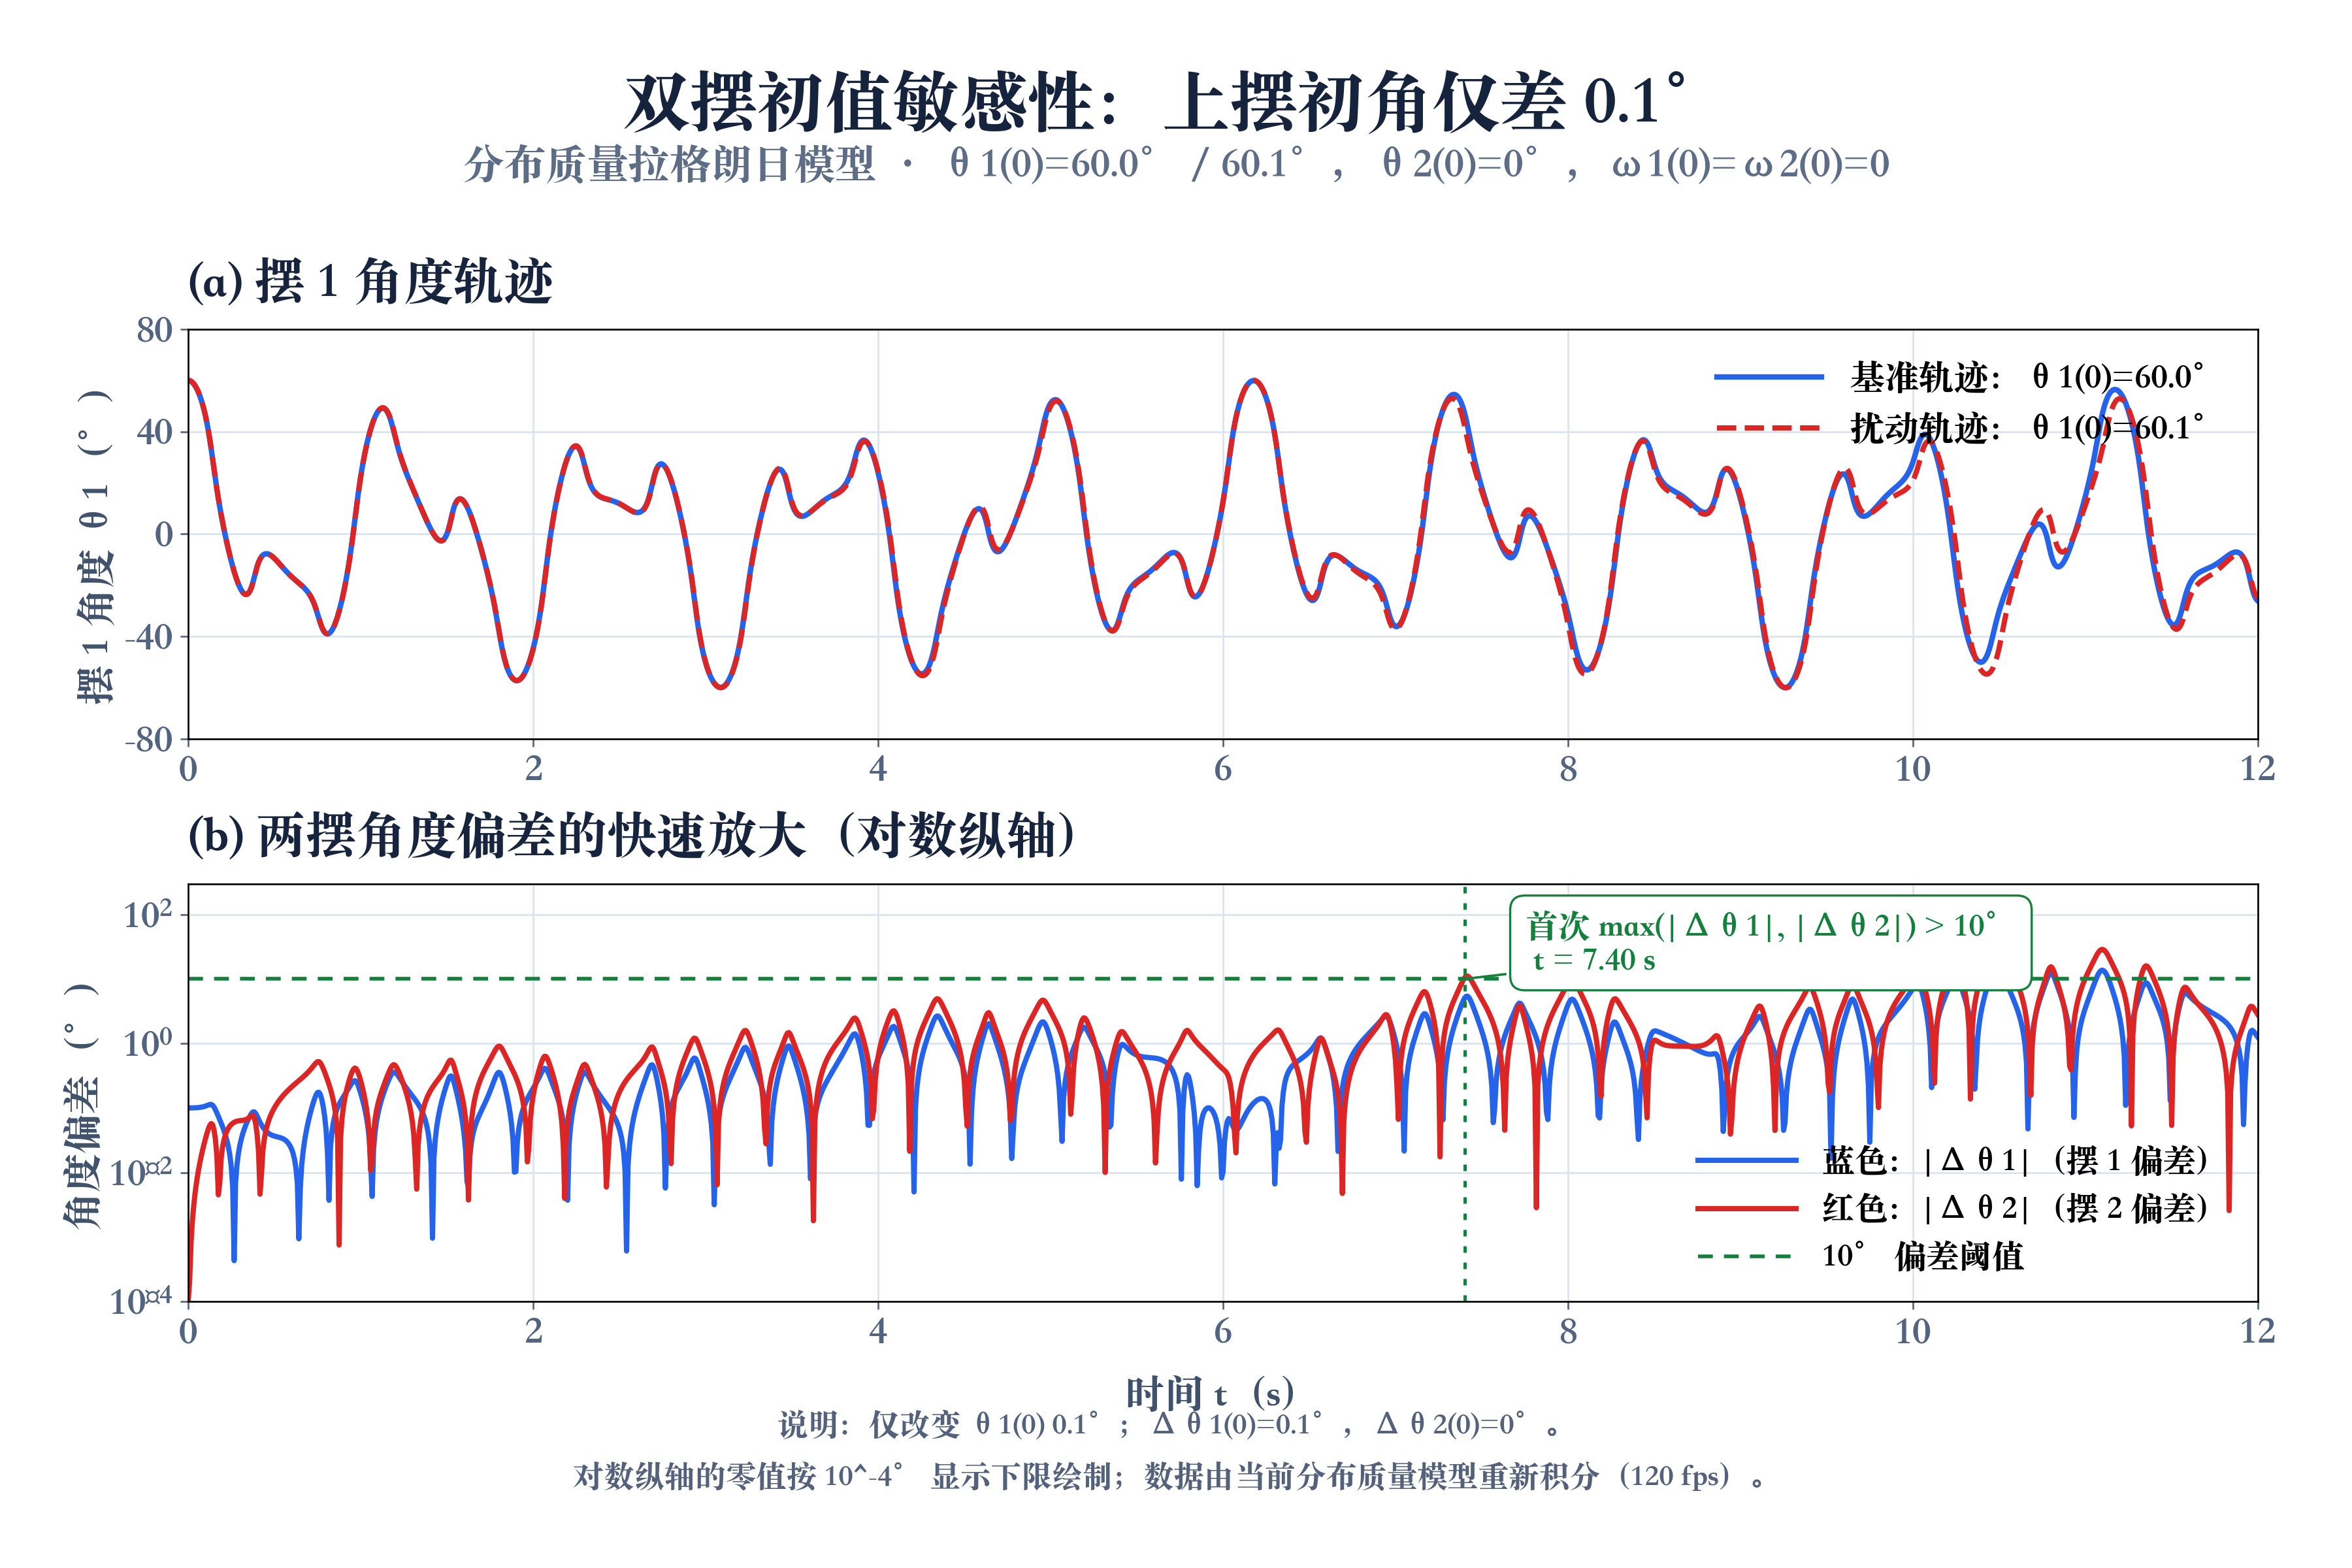
\includegraphics[width=0.98\linewidth]{../data/sim/figures/fig_butterfly_distmass_large.png}
\caption{蝴蝶效应（分布质量拉格朗日模型）：仅将 $\thetaone(0)$ 从 $60.0^\circ$ 改为 $60.1^\circ$，其余初值均保持 $\thetatwo(0)=0^\circ$、$\omega_1(0)=\omega_2(0)=0$。
(a) 两条 $\thetaone$ 轨迹前期几乎重合，随后分叉；(b) 分别给出两摆角度偏差的绝对值（对数纵轴）。初始时 $|\Delta\theta_1|=0.1^\circ$、$|\Delta\theta_2|=0^\circ$；后者的零值以 $10^{-4}\,{}^\circ$ 的显示下限绘制。首次满足 $\max(|\Delta\theta_1|,|\Delta\theta_2|)>10^\circ$ 的时刻为 $7.40\,$s。}
\label{fig:butterfly}
\end{figure}

% =============================================================================
\section{实验装置}
\label{sec:apparatus}

\subsection{机械设计}
装置正视装配图见仓库 \texttt{diagrams/02\_mechanical\_front\_view.svg}，
关键尺寸与材料：
\begin{itemize}[leftmargin=2em]
  \item 摆长：$L_1 = 250$\,mm，$L_2 = 200$\,mm（非对称避免简正模退化）
  \item 摆臂：6061-T6 铝板，$4$\,mm 厚（匹配 MR105ZZ 轴承宽度 4\,mm）
  \item 主轴承：MR105ZZ 微型深沟球轴承，工业酒精脱脂去除厂润滑脂，单滴 MOEBIUS 9020 钟表油重新润滑
  \item 配重盘：45\# 碳钢 $\varnothing 30 \times 12$\,mm，$66$\,g
  \item 主轴座：6061-T6 5\,mm 厚，$\varnothing 5$ H7 轴孔 + 2 个 M5 安装孔
  \item 框架：$2020$ 国标铝型材，T 槽螺母拼接
\end{itemize}
材料 + 加工件 + 视觉件总采购成本约 580 元（详 \texttt{diagrams/parts/BOM.md}）；
其中背板与标记两项视觉件按设计方案计入，实拍 29 段实际采用的是更易得的替代方案（见 \cref{sec:vision}）。

\subsection{初值设定与不确定度}
本研究的真实轨迹由手动将下摆抬至目标角度后释放产生，释放角度不作精确机械控制。
关键在于：每段真实轨迹输入模型的初始状态 $(\thetaone, \thetatwo, \omega_1, \omega_2)$ 并非取自释放动作的标称角度，
而是由视觉追踪从释放后的引入窗中反演得到（见 \cref{sec:vision} 与 \cref{sec:sim2real-horizon}）。
因此模型预测所依赖的是\emph{初始状态的视觉估计精度}，而非释放动作的机械重复性——
手动释放引入的微小初始角速度也被追踪如实捕获，一并纳入初始状态。
\cref{sec:sim2real-decomp} 的误差分解实测该初值状态估计噪声为角度 $\sigma_\theta \approx 0.45^\circ$、
角速度 $\delta\omega \approx 0.09$\,rad/s，约相当于 $\pm 0.5^\circ$ 量级；
该不确定度对预测视界的影响经敏感性扫描（\cref{sec:results-sensitivity}）量化：
在该量级下 PINN 中位视界退化约 $10\%$，本文结论不受影响。

\subsection{衰减测试}
为保证机器学习训练所需的“干净”混沌窗口，装置主轴承应满足单摆 $30^\circ$ 释放衰减时间常数
$\tau \geq 30$\,s。脱脂 + 钟表油润滑方案的衰减指标由下文实物测试直接验证。
实物衰减测试已完成：单摆 $90^\circ$ 释放、重复两次，振幅自 $90^\circ$ 衰减至约 $1\text{--}2^\circ$ 历时约 $551$\,s（两次分别 $552.0$ / $550.8$\,s，重复性 $0.2\%$）；按指数包络 $A(t) = A_0 e^{-t/\tau}$ 估算等效衰减时间常数 $\tau \approx 130$\,s（随终止振幅取值在 $122\text{--}145$\,s 区间），约为设计目标的 $4$ 倍，满足 $\tau \geq 30$\,s（实测在 $90^\circ$ 大幅释放下进行、含较强空气阻力，相对 $30^\circ$ 设计口径为保守下界，$30^\circ$ 释放的 $\tau$ 只会更大）。该等效 $\tau$ 对应单摆主轴承等效粘性 $b \approx 2 I_{\mathrm{eff}} / \tau \approx 1.7 \times 10^{-4}$\,N$\cdot$m$\cdot$s/rad（手计时等效估计，$90^\circ$ 大幅释放含较强空气阻力，为保守上界）。\emph{双摆运行工况}下的关节阻尼则另由 16 段实测追踪轨迹按能量耗散率法拟合（\texttt{sim/fit\_damping.py}，详见 \cref{sec:sim2real-decomp}），分离为粘性 $b \approx 1.66 \times 10^{-5}$ 与二次空气阻力 $c \approx 8.72 \times 10^{-6}$（空气阻力约占总耗散 $78\%$，逐段 $R^2$ 实测在 $0.95\text{–}0.999$ 区间、中位 $0.986$，见 \texttt{data/sim\_damped/fit\_damping\_report.csv}）。
对单摆等效转动惯量 $I_{\mathrm{eff}} \approx 1.1 \times 10^{-2}$\,kg$\cdot$m$^2$，
$\tau \geq 30$\,s 目标对应阻尼系数上界 $b \leq 2 I_{\mathrm{eff}} / (30\,\text{s}) \approx 7 \times 10^{-4}$\,N$\cdot$m$\cdot$s/rad（实测等效 $b \approx 1.7 \times 10^{-4}$ 在此上界之内）。
我们在 \texttt{sim/baseline\_damped.py} 中实现了带粘性 + 二次空气阻力两项的仿真版本作为 \emph{v3 真值}，
默认即采用上述实测拟合系数 $b \approx 1.66 \times 10^{-5}$、$c \approx 8.72 \times 10^{-6}$（不再用占位值），亦可经命令行参数覆盖。

% =============================================================================
\section{视觉测量系统}
\label{sec:vision}

\subsection{相机配置}
采用消费级智能手机后置摄像头以 $60$\,fps 拍摄（数据集统一采用 60\,fps 长时连续录像；
机型亦支持 120\,fps 慢动作，仅用于早期测试，未纳入分析数据集）。
本装置下摆的小摆动频率按点质量近似为 $\sqrt{g / L_2}/2\pi \approx 1.1$\,Hz；混沌大幅甩动下的瞬时角速率远高于此。
由 29 段正式追踪结果（\texttt{data/tracking/tracked\_*.csv}，共 $411\,746$ 帧）回算，
$\max(|\omega_1|, |\omega_2|)$ 的全库峰值为 $25.8$\,rad/s，折合 $4.11$\,Hz；
逐段峰值的中位为 $3.19$\,Hz，折合频率超过 $3.2$\,Hz 的帧仅占 $0.04\%$。
以实测全库峰值 $4.11$\,Hz 计，$60$\,fps 约为 $15$ 倍过采样（相对 $8.2$\,Hz 的 Nyquist 采样下限约为 $7$ 倍）；
该峰值处单帧角度增量约 $24.7^\circ$，远小于相位解卷绕失效所需的 $180^\circ$，采样充分。
相机固定于三脚架，光轴近似垂直于摆动平面，录制分辨率 $1920 \times 1080$；
由标定内参（$f_x / W \approx 0.81$，水平视场角约 $63^\circ$）与下述像素标度反推，工作距离约 $0.9$\,m。
以正式 29 段追踪结果中 $m_1$--$m_2$ 像素间距的中位（$353$\,px）对下摆长 $L_2 = 200$\,mm 定标，
得有效像素标度约 $0.57$\,mm/px，对应视野约 $1.1 \times 0.6$\,m。

\subsection{追踪算法}
上下摆铰接处与下摆末端各贴一枚方形彩色贴片作为视觉标记：铰接处记 $m_1$（蓝色），末端记 $m_2$（浅红色）；
两枚标记在实拍打光下均无镜面高光，末端标记成像偏粉、饱和度偏低。
正式 29 段中 $m_1$、$m_2$ 的连通域面积中位分别约 $370$ 与 $650$\,px，按上述 $0.57$\,mm/px 折合等效直径约 $12$ 与 $16$\,mm。
拍摄背景为置于摆后方的深色织物，画面两侧仍可见浅色墙面。
\texttt{diagrams/parts/BOM.md} 中列出的哑光黑亚克力背板与 $\varnothing 5$\,mm 反光圆点标记属装置设计方案，
本文 29 段实测录像未采用，正文各处均以上述实拍状态为准。
实拍追踪管线（\texttt{tracking/track\_pendulum.py}）流程：
\begin{enumerate}[leftmargin=2em]
  \item 帧 BGR 色彩通道（蓝、绿、红）$\to$ HSV 色彩空间（色相、饱和度、明度）
  \item 红色区间 + 蓝色区间各自做 \texttt{inRange} 阈值分割（红色由于跨越 H=0$^\circ$ 用双段并集）
  \item 形态学开 + 闭运算（半径 5 的椭圆核）去噪
  \item \texttt{connectedComponentsWithStats} 取全部面积超过 \texttt{MIN\_AREA} 的连通域作为候选
        （合成视频验证脚本 \texttt{track.py} 在此直接取最大连通域）
  \item 像素轨迹 $\to$ 物理坐标（自动标定：$m_1$ 轨迹最小二乘拟合圆得支点与 $L_1$ 像素半径）
  \item 反解角度：$\thetaone = \mathrm{atan2}(x_1, -y_1)$，$\thetatwo = \mathrm{atan2}(\Delta x, -\Delta y)$
\end{enumerate}
保留全部候选、再交由双向 Viterbi 选轨，是本管线与逐帧取最大连通域这一常见做法的主要差别。实拍画面中的同色干扰并不罕见：作为背景的深色织物在相机中成像偏藏青、色相落入蓝色区间——若仅把明度门限退回脚本默认（\texttt{-{}-blue-vmin 40}，饱和度与空间门限仍取正式参数），$29$ 段每帧的蓝候选中位便涨到 $27\text{--}76$ 个（全库中位 $41$ 个，其中 IMG\_1448 段为 $46$ 个，与下文消融一致；逐段统计见 \texttt{tools/count\_blue\_candidates.py}，结果落盘于 \texttt{data/tracking\_ablation/}），织物褶皱与底边缝线处尤其容易形成不随摆动移动的常驻斑点，面积有时还大于真标记；暖色墙面与释放瞬间入镜的手则会落进红色阈值。其中个别干扰恰好还位于距末端标记约 $\ell$ 处——此时仅凭刚性距离无从判别。我们在 IMG\_1448 段（$13\,153$ 帧）上对选轨策略做了消融（\texttt{tools/ablation\_transition\_cost.py}，两种策略共用同一批检测候选，差别仅在转移代价系数）：沿用脚本默认的低明度门限时，每帧蓝候选中位达 $46$ 个（最多 $67$ 个），只用刚性距离约束有 $9\,123$ 帧（$69\%$）选到与联合判别不同的候选，$m_1$ 圆拟合 RMS 残差为 $133$\,px；补上帧间位移的转移代价后残差降至 $43$\,px。但二者均远超下文 $10$\,px 的合理性门槛，说明时序连续性能大幅压制同色假阳性、却并不能挽救一个取错的阈值——这正是本管线在阈值标定之外还要设硬性合理性检查的原因。而在抬高明度门限后的正式参数下，每帧蓝候选中位降至 $1$ 个、仅 $9$ 帧出现多候选，两种策略选出的轨迹完全一致（RMS 均为 $0.42$\,px），此时刚性约束已单独够用。可见转移代价的价值随假阳性密度而变，两条准则联合使用才能在参数偏离时仍保持鲁棒。

阈值随场景标定：正式数据集 29 段共用同一套 HSV 阈值（蓝色明度门限 $V \geq 160$、饱和度门限 $S \geq 55$ 与右侧空间门限），仅时间窗逐段不同；抬高蓝色明度门限正是为了把偏藏青的背景与实测明度约 $240$ 的高亮蓝标分开。阈值取错时管线不会报错，而会给出自洽却错误的结果（命中率与帧间平滑度等内建指标仍全部正常，支点却被拟合到画面之外），故在写出结果前设三项硬性合理性检查：支点须落在画面内、圆拟合 RMS 残差须 $\leq 10$\,px、$\ell / r$ 须落在设计值 $L_2 / L_1 = 0.80$ 的 $\pm 25\%$ 以内，任一不满足即拒绝写盘。29 段的完整复现命令留档于 \texttt{tracking/reproduce\_29.sh}，据此重跑所得 CSV 与本文所用追踪结果逐字节一致（已抽取其中 5 段核对 MD5）。脚本另备一条 Lab 色彩空间的检测分支（\texttt{-{}-detector lab}）以适配不同配色的标记，本文 29 段数据全部采用上述 HSV 分支。

角度定义与几何反演的精度在 \texttt{data/sim/figures/anim\_trial\_000.mp4}（30\,fps 合成动画，真值已知）上验证——该合成片段由 \texttt{tracking/track.py} 追踪，与实拍脚本共用同一套角度定义与自动标定几何——跟踪角度中位误差
$\thetaone : 0.12^\circ$, $\thetatwo : 0.15^\circ$，$90\%$ 分位误差 $0.25\text{--}0.35^\circ$。
该结果表明追踪算法在干净图像上误差极小；真实拍摄下初值状态的估计噪声更高（约 $0.45^\circ$，见 \cref{sec:sim2real-decomp}），主要来自实拍光照、反光与运动模糊，构成真实视界的主要可改进来源之一。

\subsection{标定与精度}
相机内参用 OpenCV 的 \texttt{calibrateCamera} \cite{bradski2000}（基于 Zhang 平面标定法 \cite{zhang2000}）在 7$\times$9 棋盘格上标定。
仓库内存有两套标定：29 段 canonical 追踪结果由 \texttt{camera\_params.npz}（五参畸变模型）产出，
这也是 \texttt{tracking/track\_pendulum.py} 默认加载的标定；此外还有一次后做的重标定
\texttt{camera\_params\_新标定.npz}（14 张有效标定图，固定 $k_3 = 0$ 的四参模型，平均重投影误差 $0.44$\,px），
未用于产出本文数据。为确认结论不依赖标定的选取，我们把两套标定分别作用于 29 段的标记点轨迹并反演角度
（\texttt{tools/calib\_sensitivity.py}）：扣除两者主点差异造成的整体常数偏置后，
逐帧角度残差的逐段中位为 $\thetaone\,0.10^\circ$、$\thetatwo\,0.22^\circ$，
均小于约 $\pm 0.5^\circ$ 的初值状态估计不确定度（\cref{sec:sim2real-decomp}），故标定选取对本文结论无实质影响。
摆的运动平面与相机光轴近似垂直，且角度反演只取像素差的比值、与整体像素标度无关，
因此无须把像素轨迹换算为米制即可得到角度。实测亦支持这一处理：29 段中 $m_1$--$m_2$ 像素间距在整段内的
相对波动（标准差/中位）中位为 $1.2\%$、最大 $1.6\%$，说明投影标度全程近似恒定，
面外运动与透视效应造成的标度变化处于同一量级。

% =============================================================================
\section{机器学习模型}
\label{sec:ai-models}

\subsection{回声状态网络（ESN）基线}
\label{sec:esn}
ESN 的核心思想是用稀疏随机循环网络（“储池”）将输入投影到高维非线性
特征空间，仅训练线性读出层 \cite{jaeger2004}。本研究 ESN 配置：
\begin{itemize}[leftmargin=2em]
  \item 储池规模 $N_{\mathrm{res}} = 800$
  \item 谱半径 $\rho(\bm{W}) = 0.95$（接近临界，满足回声状态性质）
  \item 漏率 $= 0.25$，稀疏度 $0.1$
  \item 输入编码：状态 $(\thetaone, \omega_1, \thetatwo, \omega_2)$ 映射为
        $(\sin\thetaone, \cos\thetaone, \omega_1 / 10, \sin\thetatwo, \cos\thetatwo, \omega_2 / 10)$
        6 维向量
  \item 读出层用岭回归 $\alpha = 10^{-5}$ 求解，washout 200 步
\end{itemize}
\noindent 上述为仿真侧配置。真实数据侧每段仅有 $4$\,s 引入窗可供自训练，
为避免小样本下的过拟合，ESN 基线改用规模更小的储池（$N_{\mathrm{res}} = 300$、漏率 $0.3$、
$\alpha = 10^{-3}$、washout $50$，见 \texttt{rc/real\_validation\_multi.py}）。
为排除“人为削弱基线”的疑虑，我们把上述仿真侧配置连同一个四因子超参网格
（储池规模、谱半径、漏率、岭系数）同样在 29 段真实数据上完整跑过一遍
（\texttt{tools/esn\_grid\_real.py}，结果见 \texttt{data/esn\_grid\_real/summary.md}）：
在本文所用的 $4$\,s 引入窗下，仿真侧配置给出的 ESN 中位视界为 $\ge 0.167$\,s、
网格最优配置为 $\ge 0.183$\,s（“$\ge$”因部分片段右删失，中位为下界），
均仍显著低于同一单次运行口径下的 PINN $0.417$\,s 与 Hybrid $0.484$\,s
（seed 42，\texttt{data/real\_validation/summary\_multi.csv}；\cref{tab:real-horizon} 报的是 8 次独立重训的逐次运行中位）；
作为同口径参照，真实侧配置本身在该网格下为 $\ge 0.150$\,s。可见本文结论不依赖 ESN 配置的选取。

\paragraph{物理先验的优势边界：引入窗越长，纯数据基线越强} 同一份网格扫描还沿引入窗长度
$T_{\mathrm{lead}} \in \{2, 4, 8, 16, 32\}$\,s 做了二维展开，回答一个自然的追问——
纯数据 ESN 需要每段多少秒实测数据现场自训练，才能追平一秒真实数据都不用的零样本物理模型。
在预测窗同为 $4$\,s 的口径下，网格最优 ESN 的中位视界随 $T_{\mathrm{lead}}$ 由 $0.150$\,s（$2$\,s）
增至 $\ge 0.183$（$4$\,s）、$\ge 0.534$（$8$\,s）、$\ge 1.234$（$16$\,s）、$\ge 3.735$\,s（$32$\,s），
而 Hybrid 相应为 $0.600 / 0.484 / 0.717 / 1.000 / 1.267$\,s：
在本文所用的 $4$\,s 引入窗下物理先验占优约 $2.6$ 倍，$T_{\mathrm{lead}} = 16$\,s 附近纯数据基线反超，
$32$\,s 时已明显领先。我们如实报告这一交叉，并据此把本文的结论限定在其成立的条件上：
\emph{物理先验的价值出现在真实数据稀缺的一侧}——每段只有数秒可用历史时，
把已知方程放进模型远比让网络从这几秒里学动力学更有效；一旦每段可获得数十秒的实测数据，
纯数据方法自会追上并超过。这正是低成本、短录制场景（也是本文的目标设定）最关心的区间。
需说明的是，长引入窗档的中位数受右删失影响较大（$T_{\mathrm{lead}} = 32$\,s 时删失率达 $48\%$），
其数值为下界，故上述交叉点的位置只宜作量级判断。逐档完整结果见 \texttt{data/esn\_grid\_real/summary.md}。
完整实现见 \texttt{rc/esn.py}（约 290 行）。

\subsection{物理-数据混合模型（Hybrid）}
\label{sec:hybrid}
为评估“已知物理 + NN 残差”范式在本任务上的价值，我们实现了
Universal Differential Equation 风格的 Hybrid 模型 \cite{rackauckas2020universal}：
\begin{equation}
\dot{\bm{\omega}}_{\mathrm{Hybrid}}(\bm{\theta}, \bm{\omega})
= \dot{\bm{\omega}}_{\mathrm{baseline}}(\bm{\theta}, \bm{\omega}) + s \cdot \mathrm{MLP}(\bm{\theta}, \bm{\omega})
\label{eq:hybrid}
\end{equation}
其中 $\dot{\bm{\omega}}_{\mathrm{baseline}}$ 为 \cref{eq:eom} 给出的解析方程右端项（right-hand side, RHS），
$s$ 为残差缩放因子。MLP 末层权重采用 \texttt{xavier\_normal} 初始化（$\mathrm{gain}=0.01$），并取很小的初始幅度，
保证初始预测约等于解析先验。Hybrid 的训练损失与 PINN 同构（\cref{eq:pinn-loss}），
同为数据项与拉格朗日物理残差项的加权和，取 $\lambda_{\mathrm{phys}} = 0.5$、配点数 $1024$、
batch $512$、Adam 学习率 $1 \times 10^{-3}$ 配余弦衰减，训练 $200$ epoch。
因解析先验已承担右端项的主体，网络只需学一个很小的残差，物理残差项在训练早期即接近零；
该权重在此的作用是约束残差不把解推离物理可行流形，而非像 PINN 那样承担物理信息的主要注入。
完整实现见 \texttt{rc/hybrid.py}。

\subsection{物理约束神经网络（PINN）}
\label{sec:pinn}

\paragraph{网络结构} MLP，6 维输入 $\to$ 128 单元 $\times 4$ 隐层 $\to$ 2 维输出（$\dot\omega_1, \dot\omega_2$）。
输入采用极坐标编码 $(\sin\theta_i, \cos\theta_i, \omega_i / W_{\text{scale}})$，
输出归一化 $\dot\omega / A_{\text{scale}}$，其中 $W_{\text{scale}} = 10$，$A_{\text{scale}} = 100$。

\paragraph{损失函数} 数据项 + 物理项的加权和
\begin{equation}
\mathcal{L} = \mathcal{L}_{\text{data}} + \lambda_{\text{phys}} \, \mathcal{L}_{\text{phys}}
\label{eq:pinn-loss}
\end{equation}
其中物理残差直接从 \cref{eq:eom} 推出
\begin{equation}
\mathcal{L}_{\text{phys}} = \left\| \bm{M}(\bm{\theta}_c) \, \dot{\bm{\omega}}_{\text{NN}}(\bm{\theta}_c, \bm{\omega}_c)
- \bm{b}(\bm{\theta}_c, \bm{\omega}_c) \right\|^2
\end{equation}
每个 epoch 均重新采样 2048 个配点（即用于计算物理残差的状态点）$(\bm{\theta}_c, \bm{\omega}_c)$。

\paragraph{训练} 训练 300 个 epoch（完整遍历训练集的轮次），采用 Adam（自适应矩估计）优化器，初始学习率为 $2 \times 10^{-3}$，并使用余弦衰减。
\cref{alg:pinn-train} 给出完整训练流程。

\begin{algorithm}[h]
\caption{PINN 训练循环（rc/pinn.py 实现）}
\label{alg:pinn-train}
\begin{algorithmic}[1]
\Require 训练数据 $\{(\bm{s}^{(i)}, \dot{\bm{\omega}}^{(i)})\}_{i=1}^N$（来自 trial 0-4 前 20\,s）
\Require 网络 $f_\phi : \mathbb{R}^4 \to \mathbb{R}^2$，损失权重 $\lambda_{\mathrm{phys}}$，配点数 $N_c$
\Ensure 训练后的网络参数 $\phi^*$
\For{epoch $= 1$ \textbf{to} $300$}
  \For{每个 mini-batch $\mathcal{B}$（batch size 512）}
    \State 从训练集采样 $(\bm{s}_b, \dot{\bm{\omega}}_b) \in \mathcal{B}$
    \State 从相空间 $\bm{\theta} \in [-\pi, \pi]^2,\ \omega_1 \in [-20, 20],\ \omega_2 \in [-25, 25]$ 均匀采样 $N_c = 2048$ 个配点 $\{\bm{s}_c\}$
    \State $\dot{\bm{\omega}}_b^{\mathrm{pred}} \gets f_\phi(\bm{s}_b)$；\quad $\dot{\bm{\omega}}_c^{\mathrm{pred}} \gets f_\phi(\bm{s}_c)$
    \State $\mathcal{L}_{\mathrm{data}} \gets \| (\dot{\bm{\omega}}_b^{\mathrm{pred}} - \dot{\bm{\omega}}_b) / A_{\mathrm{scale}} \|^2$
    \State $\mathcal{L}_{\mathrm{phys}} \gets \| \bm{M}(\bm{\theta}_c) \, \dot{\bm{\omega}}_c^{\mathrm{pred}} - \bm{b}(\bm{\theta}_c, \bm{\omega}_c) \|^2$
    \State $\mathcal{L} \gets \mathcal{L}_{\mathrm{data}} + \lambda_{\mathrm{phys}} \cdot \mathcal{L}_{\mathrm{phys}}$
    \State $\phi \gets \mathrm{Adam}(\phi, \nabla_\phi \mathcal{L})$
  \EndFor
  \State 更新余弦学习率
\EndFor
\State \Return $\phi$
\end{algorithmic}
\end{algorithm}

\paragraph{闭环预测} 用 RK4（四阶 Runge--Kutta 法）积分 $\dot{\bm{s}} = [\omega_1, \dot\omega_1, \omega_2, \dot\omega_2]$，
$\dot{\bm{\omega}}$ 由训练好的 $f_{\phi^*}$ 给出，时间步 $\Delta t = 1/120$\,s。

% =============================================================================
\section{结果与分析}
\label{sec:results}

\subsection{评测协议}
\label{sec:results-protocol}
全文以\emph{可信预测视界}为唯一评测指标，定义为闭环预测的角度偏差首次超过阈值的时刻
\begin{equation}
h = \min\left\{ t \;:\; \sqrt{\Delta\thetaone(t)^2 + \Delta\thetatwo(t)^2} > 10^\circ \right\},
\quad
\Delta\theta_i = \mathrm{atan2}\!\left(\sin\delta_i,\, \cos\delta_i\right),\;
\delta_i = \hat\theta_i - \theta_i
\label{eq:horizon}
\end{equation}
其中 $\hat\theta_i$ 为预测角，$\theta_i$ 为解析积分或视觉追踪给出的真值角；$\mathrm{atan2}$ 形式用于消除角度的
$2\pi$ 周期歧义。若整个评估窗内偏差始终不超阈，则记视界为窗长并标注为\emph{右删失}，该值为真实视界的下界。
仿真内与真实数据两侧共用同一实现，仅评估窗长不同（仿真 $10$\,s、真实 $4$\,s）。
\cref{fig:butterfly} 的蝴蝶效应示意为便于逐轴读图另用 $\max(|\Delta\thetaone|, |\Delta\thetatwo|) > 10^\circ$ 判据，
其 $7.40$\,s 与本节各表不属同一口径，不作横向比较。$10^\circ$ 阈值本身的稳健性核验见 \cref{sec:appendix-honesty}。

\subsection{可信预测视界}
\label{sec:results-horizon}

仿真内的训练与评测按如下口径划分：PINN、纯数据 MLP 与 Hybrid 三者仅以 trial 0--4 前 $20$\,s 的
状态与加速度样本训练一次，随后在全部 50 组随机初值（trial 0--49）第 $20$\,s 处以真值状态为起点闭环外推 $10$\,s，
其中 45 组为训练中未出现过的轨迹；ESN 则是逐段自训练的时序模型，对每个 trial 单独以其前 $20$\,s
训练读出层，再预测同一 trial 随后的 $10$\,s。此口径对 ESN 有利——它拿到的是待预测轨迹本身的历史，
而三个网络模型只拿到一个初始状态；物理先验模型在此不利口径下仍占优。
需说明的是，trial 0--4 的预测段虽与其训练段在时间上不重叠，但仍取自训练所用的同一批轨迹，
故 50 组评测中有 5 组并非严格的样本外评估。
每个模型均在自身的混沌子集（视界 $< 9.9$\,s）上取中位数，以排除少数落入或被预测为长周期轨道的试验样本（trial）；
其中三方模型（ESN / PINN / Hybrid）一致判定为混沌的样本共 $N = 32$（\cref{fig:three-way} 所用子集）。
统计结果列于 \cref{tab:horizon-compare}。

\begin{table}[h]
\centering
\caption{50 组完整扫描 · 混沌 trial（每次运行取视界 $< 9.9$\,s 子集）闭环预测视界统计（$10^\circ$ 阈值）。
每个模型独立训练多次（ESN 更换储池随机种子 $\times 10$；PINN/Hybrid 非确定性重训 $\times 8$），报告逐次运行中位的中位数及四分位距 [IQR]。}
\label{tab:horizon-compare}
\begin{tabular}{lcccc}
\toprule
模型 & 视界中位 (s) & IQR (s) & 归一化 $/\tauL$ & 相对 ESN \\
\midrule
ESN（数据驱动基线）            & 0.70 & [0.55,\,0.70] & 0.91 & 1.0$\times$ \\
PINN（$\lambda_{\text{phys}}{=}0.1$） & 0.88 & [0.77,\,1.03] & 1.15 & 1.3$\times$ \\
纯数据 MLP（$\lambda_{\text{phys}}{=}0$，消融） & 1.55 & [1.31,\,1.68] & 2.03 & 2.2$\times$ \\
Hybrid（解析先验$+$残差）       & 2.85 & [2.12,\,3.27] & 3.74 & 4.1$\times$ \\
\bottomrule
\end{tabular}
\\[1em]
\footnotesize 倍数为各模型逐次运行中位数之比。Hybrid 与纯数据 MLP 明显超过数据驱动的 ESN 基线，
PINN 亦高于 ESN 但幅度有限；其中解析先验最完整的 Hybrid 在仿真内最强。
带物理损失的 PINN（$\lambda{=}0.1$）仿真内中位（0.88\,s）低于无物理损失的纯数据 MLP（1.55\,s）——
在干净、无噪的仿真数据上纯数据拟合本就最准，物理损失在此略有代价；其真正价值体现在
sim$\to$real 零样本迁移（见 \cref{sec:sim2real-decomp}）。
\emph{ESN 行取修正后的值}：早先的闭环实现中，预测入口的储池起跑点与训练契约相差一个储池步——
训练时状态 $\bm{X}[t]$ 已消费输入 $\bm{U}[t]$，而闭环入口又把该帧重喂了一次——
致使 ESN 在预测窗第 $0$ 帧即带约 $2^\circ$ 的角度偏差（修正后降至 $10^{-3}$ 度量级），
中位视界被压至 $0.40$\,s。按训练契约对齐起跑点后 ESN 升至 $0.70$\,s，
相对倍数相应由 $2.2 / 3.8 / 7.0$ 修正为 $1.3 / 2.2 / 4.1$。
新旧实现的逐位等价验证与逐 trial 对照见 \texttt{tools/esn\_closedloop\_fix.py}。
真实侧的 ESN 调用本就与训练契约一致，\cref{tab:real-horizon} 的数字不受影响。
\end{table}

\noindent 以自测 $\tauL = 0.76$\,s 归一化，纯数据驱动的 ESN 可维持约 $0.91\,\tauL$ 的可信预测——
这与文献给出的“约 $1$--$2$ 个 Lyapunov 时间”的储池计算基线相符 \cite{lu2017reservoir,pathak2018}，
表明本文的 ESN 基线处于合理水准而非被削弱；
引入物理结构后，Hybrid 视界扩展到约 $3.7\,\tauL$（相对 ESN 约 4.1 倍），纯数据 MLP 约 $2.0\,\tauL$（2.2 倍），
带拉格朗日物理损失的 PINN 约 $1.2\,\tauL$（1.3 倍）。物理先验模型相对 ESN 的提升是本研究在仿真内的核心结论，
独立于 $\tauL$ 的绝对值估算。所有数字均为多次独立训练得到的逐次运行中位数及四分位距，以反映训练随机性。
三方完整分布如 \cref{fig:three-way} 所示。

\begin{figure}[H]
\centering

\includegraphics[width=\linewidth]{three_way_compare.png}
\caption{ESN / PINN / Hybrid 三方对比三联图。(a) 三方视界箱线图（对数纵轴）；
(b) 经验累积分布函数（cumulative distribution function, CDF）；(c) 散点图：横轴为 ESN 视界，纵轴为 PINN / Hybrid 视界。
$N=32$ 个三方一致的混沌样本。这是固定一次训练的逐 trial 可视化，故中位数为 ESN\,$\approx$\,0.29\,s / PINN\,$\approx$\,0.51\,s / Hybrid\,$\approx$\,2.17\,s；\cref{tab:horizon-compare} 则报告多次独立训练的逐次运行中位数。两者口径不同，图中数值不用于替代表中统计。
本图的 ESN 曲线取自修正前的闭环起跑点（见 \cref{tab:horizon-compare} 脚注），仅用于展示三方视界的分布形态与逐 trial 相关性，不用于支撑任何倍数结论；按修正路径重算后 ESN 的分布整体右移，Hybrid 相对 ESN 的逐 trial 优势仍然成立。}
\label{fig:three-way}
\end{figure}

\subsection{初值精度敏感性扫描}
\label{sec:results-sensitivity}
为评估约 $\pm 0.5^\circ$ 量级的初值状态估计不确定度对预测视界的影响，
我们在 50 组仿真轨迹中取「PINN 无扰动视界 $< 9.9$\,s」的混沌子集（$49$ 组；子集在无扰动处一次定死，
跨扰动档、跨模型均不变，以保证可比），对初值施加独立高斯扰动，每档重复 $K = 20$ 次，
统计全部 trial$\times$rep 的中位视界（脚本 \texttt{tools/sensitivity\_correct.py}）。
除三个学习模型外，同时把\emph{解析真解}（以扰动后的初值积分同一组方程）纳入同一流程作为参照。
结果列于 \cref{tab:sensitivity}。

\begin{table}[h]
\centering
\caption{初值高斯扰动下的中位可信预测视界（仿真内混沌子集 $49$ 组，每档 $K=20$ 次独立扰动，单位 s）。三个学习模型均使用冻结的 canonical 权重单次评估，故本表无扰动行与 \cref{tab:horizon-compare} 的多次重训逐次运行中位属不同口径，数值不可直接比较。需特别提请注意：本表无扰动行中 PINN（1.48）高于纯数据 MLP（1.28），与 \cref{tab:horizon-compare} 的顺序相反。这是单次冻结权重评估的必然后果——两个模型在独立重训下的逐次运行中位区间高度重叠（PINN $0.68$--$1.93$\,s、MLP $1.08$--$1.93$\,s），单取一次抽样落在哪一侧都有可能。比较两者强弱应以 \cref{tab:horizon-compare} 的多次重训统计为准；本表的用途是同一组权重在不同扰动档之间的\emph{相对}退化，该用途不受此影响}
\label{tab:sensitivity}
\begin{tabular}{lcccc}
\toprule
扰动档 & PINN & MLP($\lambda{=}0$) & Hybrid & 解析真解 \\
\midrule
无扰动 & 1.48 & 1.28 & 3.69 & 10.00 \\
\midrule
\multicolumn{5}{l}{\emph{角度扰动} $\sigma_\theta$} \\
\quad $0.1^\circ$ & 1.43 & 1.28 & 3.68 & 10.00 \\
\quad $0.45^\circ$（本研究实测） & 1.38 & 1.18 & 3.33 & 4.69 \\
\quad $1.0^\circ$ & 1.15 & 1.07 & 2.35 & 2.47 \\
\midrule
\multicolumn{5}{l}{\emph{角速度扰动} $\delta\omega$（rad/s）} \\
\quad $0.03$ & 1.40 & 1.27 & 3.66 & 10.00 \\
\quad $0.09$（本研究实测） & 1.35 & 1.19 & 3.35 & 6.55 \\
\quad $0.2$ & 1.18 & 1.10 & 2.60 & 3.12 \\
\midrule
联合（$0.45^\circ$ 与 $0.09$\,rad/s） & 1.33 & 1.15 & 2.82 & 3.45 \\
\bottomrule
\end{tabular}
\end{table}

\noindent 读表需注意：解析真解是其中唯一\emph{纯净}的敏感性曲线——它在无扰动时逐位复现真值
（视界顶到 $10$\,s 的窗长上限），扰动是它唯一的误差源，故塌缩必然单调；而 PINN/MLP/Hybrid 自身带有
模型逼近误差，小扰动有时会与模型偏差部分抵消，个别档位出现视界不降反升（如 PINN 的 $\sigma_\theta$ 序列
即为非单调），不应据此认为预测对初值噪声“稳健”。

在本研究实测的联合初值不确定度（$\sigma_\theta = 0.45^\circ$、$\delta\omega = 0.09$\,rad/s）下，
PINN 中位视界由无扰动的 $1.48$\,s 降至 $1.33$\,s（$-10\%$，四分位区间 $[0.78, 2.37]$\,s），
Hybrid 由 $3.69$\,s 降至 $2.82$\,s（$-24\%$），而解析真解由 $10.00$\,s 塌至 $3.45$\,s。
三者并置给出一个明确结论：在当前初值精度下混沌放大确实在起作用（解析解的塌缩即是它的纯净度量），
但学习模型的视界主要受限于模型自身的逼近误差而非初值噪声——这也解释了为何继续提高初值估计精度
对 PINN 的边际收益有限，而对已接近真解的 Hybrid 与解析解影响显著。真实数据侧的同口径扫描给出一致结论：
PINN 逐段中位视界在联合扰动下由 $0.417$\,s 微降至 $0.400$\,s。作为口径互校，解析真解在确定性联合扰动下
对理想轨迹的视界中位为 $2.07$\,s，与 \cref{sec:sim2real-decomp} 由逐片实测噪声估得的混沌天花板
$C_{\mathrm{chaos}} = 1.90$\,s 同量级。

需要说明的是，本节结果来自 $2026$ 年 $9$ 月修正后的扰动协议。早先版本的扫描脚本调用了
未对齐的预测接口，使模型拿到的初值与它要预测的真值起点成为同一个数，扰动被逐位抵消——
模型实际看到的初值误差恒为 $0^\circ$，量到的只是 trial 间波动而非初值敏感性，
并据此得出过“视界随 $\sigma$ 增大不降反升、对初值稳健”的错误结论。诊断记录、旧协议复刻与
新旧对照见 \texttt{data/sensitivity\_correct/}（含 G1--G3 三项确定性自证门槛的通过记录）。

\subsection{Lyapunov 时间归一化}
\label{sec:results-lyapunov}
仿真内的视界除以自测中位 $\tauL = 0.76$\,s 后归一到 Lyapunov 时间单位，
该归一化使本研究结果与文献中其他混沌系统的预测窗口可直接比较，详见 \cref{tab:horizon-compare} 最右列。
真实数据侧的视界不作此归一化：$\tauL$ 由仿真轨迹的分叉率测得，而真实轨迹的能量分布与之不同，
两者除以同一常数并不增加可比性；若仍按 $\tauL = 0.76$\,s 折算，\cref{tab:real-horizon} 四个模型
分别对应 $0.22 / 0.47 / 0.55 / 0.59\,\tauL$——真实侧全部模型都还在一个 Lyapunov 时间之内，
这一点本文不回避：真实条件下的绝对可信窗口仍然很短，本文主张的是\emph{相对提升}与其成因，
而非宣称已突破混沌的可预测极限。
若改用文献高能量区的 $\tauL \approx 0.12$\,s 作归一化（更宽松的“经典”参考），
物理先验模型视界对应约 $7\text{--}24\,\tauL$，远超文献中 ESN 报告“约 $1\,\tauL$”的经典上限；
但出于保守原则，本文以自测 $\tauL$ 为准。

% =============================================================================
\section{sim$\to$real 迁移与误差成因分解}
\label{sec:sim2real}

前述视界统计均在数值仿真内部完成（训练与测试同分布）。本节检验本研究的核心命题：
在无摩擦仿真上训练的模型，能否从真实双摆的实测初值出发预测其后续运动，
以及物理约束在这种\emph{分布迁移}下是否真正有价值。

\subsection{真实数据上的三方预测视界}
\label{sec:sim2real-horizon}

我们用手机相机拍摄并经视觉追踪（\cref{sec:vision}）得到 29 段有效真实双摆轨迹
（释放角 $38^\circ$--$111^\circ$，时长 $160$--$368$\,s，均为 60\,fps）。
对每段取一个 $4$\,s 引入窗（供 ESN 自训练并为 PINN/Hybrid 提供初始状态 $\bm{s}_0$）
与随后的 $4$\,s 预测窗，按帧率无关的统一口径计算视界（仍取 $10^\circ$ 角度偏差阈值）。
PINN、纯数据 MLP 与 Hybrid 的全部权重均来自无摩擦仿真训练、未在任何真实数据上微调，
在真实段上只读取一个初始状态 $\bm{s}_0$，是严格意义的零样本迁移。
ESN 作为时序基线不适用这一约定：它的储池权重虽为随机生成、不含任何仿真或真实信息，
但其线性读出层是在每段自身的 $4$\,s 引入窗上现场岭回归拟合的，即 ESN 用到了待预测轨迹本身的真实历史。
本文保留这一非对称设置并明确标注：它对 ESN 有利而非不利，物理先验模型是在这一不利于自己的口径下仍然占优。
结果见 \cref{tab:real-horizon}。

\begin{table}[h]
\centering
\caption{29 段真实双摆轨迹上的 sim$\to$real 闭环预测视界与角度均方根误差（root mean square, RMS；$4$\,s 窗，$10^\circ$ 阈值，报告中位 [IQR]）。
视界为多次独立训练的逐次运行中位数，括号内为逐次运行四分位距；ESN 取多个储池随机种子的中位数。}
\label{tab:real-horizon}
\begin{tabular}{lccc}
\toprule
模型 & 视界 中位 (s) & 视界 IQR (s) & 预测窗角度 RMS 中位 ($^\circ$) \\
\midrule
ESN              & 0.167 & [0.167,\,0.179] & 98.2 \\
纯数据 MLP（$\lambda{=}0$） & 0.358 & [0.333,\,0.404] & --- \\
PINN（$\lambda{=}0.1$）     & 0.417 & [0.367,\,0.438] & 54.3 \\
Hybrid           & 0.450 & [0.450,\,0.467] & 51.6 \\
\midrule
PINN / ESN   & 2.5$\times$ & --- & --- \\
Hybrid / ESN & 2.7$\times$ & --- & --- \\
\bottomrule
\end{tabular}
\\[0.6em]
{\footnotesize 在 $29$ 段真实轨迹上对逐段视界进行单边配对 Wilcoxon 符号秩检验（比较配对样本的中位差异），物理先验模型显著优于 ESN：
PINN $19$/$8$ 段占优（$p = 6\times10^{-4}$）、Hybrid $20$/$7$ 段占优（$p = 4\times10^{-4}$），各 $2$ 段持平。
该检验基于逐段配对秩，不依赖中位的聚合方式。需说明口径差异：表体的四个中位取自多次独立重训的
逐次运行中位，而上述配对检验在单次运行（\texttt{seed} 42，\texttt{summary\_multi.csv}）的 29 段逐段视界上进行，
因为配对秩检验要求同一次运行内的逐段配对；两者回答的是不同问题——前者给出效应量，后者给出显著性。}
\end{table}

\noindent 与纯仿真结论一致，物理先验模型在真实数据上仍显著优于纯数据驱动 ESN：
Hybrid 与 PINN 中位视界约为 ESN 的 $2.5\text{--}2.7$ 倍，预测窗角度 RMS（$52$--$54^\circ$）远低于 ESN 的 $98^\circ$。
视界随释放角（混沌强度的代理）下降的趋势在真实数据上同样成立（\cref{fig:real-horizon}）：
29 段上视界与释放角的 Spearman 秩相关为 ESN $-0.55$、PINN $-0.46$、Hybrid $-0.47$（$p < 0.05$）。
按释放角分档还可看出，物理先验的优势随混沌强度增强而扩大——释放角 $38^\circ$--$60^\circ$ 档
三者中位为 $1.87 / 2.28 / 2.42$\,s（物理模型仅约 $1.2\text{--}1.3$ 倍），
$60^\circ$--$80^\circ$ 档为 $0.17 / 0.37 / 0.33$\,s，$80^\circ$ 以上档为 $0.14 / 0.38 / 0.47$\,s
（升至约 $2.7\text{--}3.3$ 倍）。即在越难预测的强混沌区，物理结构带来的相对收益越大；
反过来说，弱混沌区纯数据方法已足够好，物理先验的必要性也最低。
真实视界（中位约 $0.42$\,s）短于仿真内部值（PINN $0.88$\,s），其成因在 \cref{sec:sim2real-decomp} 定量分解。
真实迁移能成立的前提是仿真采用与硬件一致的\emph{分布质量}模型（\cref{sec:physics-model}）：
在理想点质量模型上训练的同款 PINN 真实中位视界仅约 $0.27$\,s，迁移质量明显更差。

\begin{figure}[H]
\centering

\includegraphics[width=\linewidth]{real_overlay_1448.png}
\caption{真实录像上的零样本预测叠加（IMG\_1448，释放角 $66^\circ$）。黑色描边的白线为视频追踪真值，
橙/绿/青分别为 ESN/PINN/Hybrid 从视频反演初值出发的闭环预测，逐帧投影回像素平面。
$t = 0$ 三模型与真值重合；$t = 0.9$\,s 数据驱动 ESN 已脱靶而物理先验模型仍贴合；
$t = 1.7$\,s 仅 Hybrid 接近真值——物理结构在真实数据上把可信预测窗口延长数倍，与 \cref{tab:real-horizon} 一致。}
\label{fig:real-overlay}
\end{figure}

\begin{figure}[H]
\centering

\includegraphics[width=\linewidth]{multi_horizon_vs_angle.png}
\caption{29 段真实轨迹上三方视界随释放角的分布。实心标记表示在 $4$\,s 窗内首次达到 $10^\circ$ 偏差；空心标记为右删失（窗口内未达阈值，取窗长为视界下界）。}
\label{fig:real-horizon}
\end{figure}

\subsection{物理损失在分布迁移下的价值}
\label{sec:sim2real-lambda}

附录 \cref{sec:appendix-ablation} 与 \cref{tab:horizon-compare} 显示，在仿真内部（同分布）物理损失权重 $\lambda_{\mathrm{phys}}$
对视界不仅无增益，甚至有损害（带物理损失 0.88\,s $<$ 纯数据 1.55\,s）——这看似削弱了物理约束的意义。
但本研究真正关心的是 sim$\to$real 的\emph{分布迁移}场景。
我们在完全相同的训练设置下（同一网络 $128\times4$、同一批仿真数据、同样 $300$ epoch、多次重训取中位），
仅令 $\lambda_{\mathrm{phys}}=0$（纯数据 MLP）与 $\lambda_{\mathrm{phys}}=0.1$（PINN，按 $\lambda$ 扫描选定）两版模型，
在上述 29 段真实轨迹上同口径对比，结果见 \cref{tab:real-lambda}。

\begin{table}[h]
\centering
\caption{真实数据上 $\lambda_{\mathrm{phys}}=0$ 与 $\lambda_{\mathrm{phys}}=0.1$ 同口径对照（29 段，$4$\,s 窗，逐次运行中位）}
\label{tab:real-lambda}
\begin{tabular}{lcc}
\toprule
 & 视界 中位 (s) & 逐段占优段数 \\
\midrule
$\lambda_{\mathrm{phys}}=0$（纯数据） & 0.36 & 10 / 29 \\
$\lambda_{\mathrm{phys}}=0.1$（PINN）  & 0.42 & 13 / 29 \\
\bottomrule
\end{tabular}
\\[0.5em]
{\footnotesize 余 6 段两者持平。\textbf{选择性说明：}$\lambda_{\mathrm{phys}} = 0.1$ 这一取值来自
一次 $\lambda \in \{0,\,0.1,\,1,\,2\}$ 的扫描，而该扫描的评价指标之一正是本表所用的同一批 29 段真实轨迹
（\texttt{data/lambda\_sweep/lambda\_sweep.csv} 的 \texttt{real} 列）。因此本表的 $1.16\times$ 属\emph{同批数据内}的
效应量估计，含选择性偏倚，应读作乐观上界而非样本外效应；要给出无偏估计，需在未参与选参的
留出片段上复测。本文不掩饰这一点：下文据此得出的结论限于\emph{方向}——物理损失的收益在分布迁移下
由负转正——而不对增益幅度作强主张。}
\end{table}

\noindent 物理损失使真实数据上的中位视界从 $0.36$\,s 提升到 $0.42$\,s（约 $1.16\times$，见上表选择性说明），
29 段中占优段数 $13$ 对 $10$。增益虽温和，但方向与仿真内部相反——这正是关键机制：
\textbf{当训练与测试同分布时，干净数据本身已足够约束解，物理损失甚至略有代价；
只有在分布迁移（sim$\to$real）下，物理先验才作为正则项防止网络外推到非物理状态而显出净收益}。
而 sim$\to$real 迁移的首要驱动仍是仿真保真度（分布质量建模），物理损失在其上提供二阶的稳健增益。
二者共同构成物理信息方法在本研究低成本实验设定中的核心价值。

\subsection{真实短视界的误差成因分解：三天花板框架}
\label{sec:sim2real-decomp}

真实视界（约 $0.42$\,s）为何短于仿真内部值？是混沌本身的不可预测性（任何模型都无能为力），
还是无摩擦模型对真实有阻尼系统的失配（我们可以改进）？我们用同口径的解析积分器隔离单一因素，
构造三条“天花板”加以定量回答（\cref{tab:three-ceiling}）：

\begin{itemize}[leftmargin=2em]
  \item $h_{\mathrm{real}}$：模型从实测 $\bm{s}_0$ 前推 vs 真实测量轨迹——实际迁移性能；
  \item $C_{\mathrm{dampmis}}$：同一初始状态下无摩擦解析积分与带阻尼解析积分的对比（拟合阻尼 $b,c$）——
        纯阻尼失配经混沌放大的天花板（完美初值）；
  \item $C_{\mathrm{chaos}}$：无摩擦解析积分分别从 $\bm{s}_0$ 与 $\bm{s}_0 + \delta$ 出发的对比——
        纯初值不确定经混沌放大的天花板（完美模型），$\delta$ 取每段实测的初值不确定度。
\end{itemize}

\begin{table}[h]
\centering
\caption{三天花板视界对比（29 段中位，$4$\,s 窗，PINN）}
\label{tab:three-ceiling}
\begin{tabular}{lcc}
\toprule
量 & 含义 & 中位 (s) \\
\midrule
$h_{\mathrm{real}}$    & 实际迁移性能                 & 0.42 \\
$C_{\mathrm{dampmis}}$ & 纯阻尼失配天花板（完美初值）   & 1.35 \\
$C_{\mathrm{chaos}}$   & 纯初值不确定天花板（完美模型） & 1.90 \\
\bottomrule
\end{tabular}
\end{table}

\noindent 实测视界 $0.42$\,s 远低于两条理论天花板（$C_{\mathrm{dampmis}} = 1.35$\,s 为其 $3.2$ 倍、
$C_{\mathrm{chaos}} = 1.90$\,s 为其 $4.5$ 倍），说明 $4$\,s 短窗内真实视界受
\emph{模型逼近误差、初值估计误差与测量噪声的组合}压制，早在阻尼失配或混沌天花板生效之前就已发散。
两点佐证：其一，用同样训练于带阻尼仿真的模型在真实数据上重测，视界并无提升
（Hybrid $0.93\times$ 基本不变，PINN 因网络外推退化反降），可见 $4$\,s 短窗内“修阻尼”无收益；
其二，初值不确定度 $\delta\omega$ 用对低阶趋势不敏感的三阶差分噪声估计器测得中位约 $0.09$\,rad/s
（对应角度测量噪声 $\sigma_\theta \approx 0.45^\circ$）。真实视界距混沌天花板尚有约 $1.5$\,s 的可改进空间，
其来源是初值状态估计精度与模型逼近能力，而非阻尼建模——这为后续改进指明了方向。
本框架与对应代码经一轮对抗式自审查校正，三处早期表述的修正记录见 \cref{sec:appendix-honesty}。

\begin{figure}[H]
\centering

\includegraphics[width=\linewidth]{error_decomposition.png}
\caption{误差成因三天花板分解（29 段真实轨迹）。(a) PINN 实测视界与两条理论天花板随释放角的分布；(b) 混沌天花板对初值不确定度 $\delta\omega$ 的敏感性，竖线为实测中位、横线为实测视界中位；(c) 实测视界、带阻尼模型视界、模型分布内上限与两条天花板的中位对比，其中带阻尼模型采用实测拟合的粘性 $b=1.66\times10^{-5}$ 和二次空气阻力 $c=8.72\times10^{-6}$；(d) 实测视界 vs 各段自身混沌天花板。}
\label{fig:error-decomp}
\end{figure}

% =============================================================================
\section{讨论与展望}
\label{sec:discussion}

\subsection{物理约束为何有效}
直觉上，纯数据驱动的 ESN 在闭环预测时仅依赖时间序列模式匹配，
对超出训练数据相空间分布的状态会产生非物理外推（违反能量守恒、动量耦合等约束），
微小预测偏差经混沌指数放大后迅速发散。
PINN 的拉格朗日物理损失
$\mathcal{L}_{\mathrm{phys}} = \| \bm{M}(\bm{\theta}_c) \dot{\bm{\omega}}_{\mathrm{NN}} - \bm{b}(\bm{\theta}_c, \bm{\omega}_c) \|^2$
在配点处强制网络输出与拉格朗日方程右端一致，
相当于在 $\dot{\bm{\omega}}$ 空间施加“流形约束”，
让外推时的解必须落在物理上可行的子流形上。
该正则化效果与 Hamiltonian 和 Lagrangian NN 的能量守恒约束秉持同一思想 \cite{greydanus2019,cranmer2020}，
但在数学形式上更为直接：即对状态方程的残差最小化。

\subsection{局限性}
\begin{itemize}[leftmargin=2em]
  \item 模型未显式建模摩擦项，长时间预测存在系统性偏差；
  \item 少数弱混沌初值下纯数据 ESN 的闭环预测在 $10$\,s 评估窗内未超 $10^\circ$ 阈值
        （视界饱和于窗长，如 trial 006/016/023），这类 trial 不计入相应模型的混沌子集；
        物理先验模型在这些 trial 上仍给出有限视界，本研究的视界对比在三方一致的完全混沌区域（$N = 32$）上最具可比性；
  \item Hybrid 解析先验的优势依赖先验与真实动力学相符：在与先验一致的无阻尼基线数据上，
        Hybrid 仿真内显著强于 PINN（中位 $2.85$\,s vs $0.88$\,s，约 $3.2\times$，\cref{sec:results-horizon}）；
        但在含未知阻尼的 \texttt{baseline\_damped} 数据上二者视界相当（单次训练中位 PINN $\approx 5.0$\,s、
        Hybrid $\approx 4.0$\,s，逐 trial 配对差异小且受训练随机性影响）——此时解析先验所基于的无摩擦模型已与真实失配，
        PINN 反而能从数据中端到端学习未建模动力学，先验不再有明显优势；
  \item sim$\to$real 迁移结果（\cref{sec:sim2real}）已用 29 段实测轨迹验证，但这些数据来自
        单台装置、主要为单次拍摄会话且均为 60\,fps；样本独立性与跨装置/跨光照/跨日的重复性
        仍有待更大规模实测进一步背书；
  \item 真实迁移为零样本（模型未在任何真实数据上微调）。引入少量真实数据做域适配或在线校正，
        有望进一步压缩 \cref{sec:sim2real-decomp} 指出的、距混沌天花板约 $1.5$\,s 的可改进空间。
\end{itemize}

\subsection{未来工作}
\begin{itemize}[leftmargin=2em]
  \item \textbf{Lagrangian Neural Network 实施挑战：} 我们在 \texttt{rc/lnn.py}
        中实现了 LNN \cite{cranmer2020}：网络学拉格朗日量 $\mathcal{L}(\bm{\theta}, \bm{\omega})$
        标量，通过自动微分计算 Hessian 矩阵（二阶导数矩阵），再反解 $\ddot{\bm{\theta}} = \bm{M}^{-1}(\bm{q})(\partial_{\bm{q}} \mathcal{L} - \bm{C} \dot{\bm{q}})$。
        简化版（Tanh MLP $128 \times 4$、余弦学习率和梯度裁剪）在本研究的基线数据上
        训练损失剧烈震荡（跨两个数量级跳变），最终视界中位数仅为 $0.08$\,s。
        Cranmer 等原工作使用更复杂的训练技巧（L-BFGS 限内存拟牛顿优化、二阶优化器、深度集成）。
        本研究列为未来工作，需进一步调优；
  \item 域适配与真实数据微调：在零样本 sim$\to$real（\cref{sec:sim2real}）基础上引入少量真实片做
        微调或在线状态估计，验证能否逼近 \cref{sec:sim2real-decomp} 的混沌天花板；
  \item 训练数据效率（见附录 \cref{sec:appendix-ablation}）；
  \item 引入阻尼项并在 50 组完整扫描上验证（已在 \texttt{baseline\_damped.py} 中实现框架）。
\end{itemize}

\subsection{应用前景}
本文在双摆这一最小试验台上得到的结论，对更广的工程动力系统预测具有直接借鉴意义。将拉格朗日力学作为先验嵌入网络的深度拉格朗日网络（Deep Lagrangian Networks）已在真实机械臂上实现更少样本、更强外推的动力学建模与实时控制 \cite{lutter2019delan}，与本文 PINN 与 Hybrid 所用的物理约束思路一脉相承；在电力系统中，融合摆动方程等物理约束的神经网络被用于电网暂态稳定与动态轨迹的快速预测 \cite{huang2023pinnpower}，其本质同样是对高维非线性系统的可信预测。储池计算仅训练读出层的特性使其易于低功耗硬件实现，已在光子、忆阻器等物理器件上得到验证 \cite{tanaka2019physical}，为本文 ESN 基线在边缘计算场景中的部署提供了现实路径。

% =============================================================================
\section{结论}
\label{sec:conclusion}

本文以一台总成本约 $580$ 元的本科实验室级双摆装置为试验台，把物理先验按由无到有、由弱到强
分为四档，在同一套数据与评测口径下量化了它对混沌可信预测窗口的贡献，得到三条结论。

\textbf{其一，物理结构的价值在仿真内即可量化，但强弱分明。} 以自测 $\tauL = 0.76$\,s 归一化，
纯数据 ESN 基线维持约 $0.91\,\tauL$（$0.70$\,s），与文献报告的储池计算水准相当；
解析先验最完整的 Hybrid 达 $3.74\,\tauL$（$2.85$\,s，约 $4.1$ 倍），
而仅以损失项施加弱约束的 PINN 只有 $1.15\,\tauL$（$0.88$\,s，$1.3$ 倍）。
起作用的主要是\emph{把已知方程直接放进模型结构}，而非把它写成一个正则项。

\textbf{其二，物理损失的价值出现在分布迁移处，而非同分布拟合处。} 在干净的同分布仿真数据上，
物理损失反而略有代价（$0.88$\,s $<$ 纯数据 MLP 的 $1.55$\,s）；而在 29 段真实轨迹的零样本
sim$\to$real 迁移中，同一对模型的中位视界由 $0.36$\,s 升至 $0.42$\,s，方向发生反转
（该幅度含选参偏倚，见 \cref{sec:sim2real-lambda}）。真实迁移中物理先验模型的中位视界为
ESN 的 $2.5\text{--}2.7$ 倍，逐段配对检验显著（$p < 10^{-3}$）。
迁移能否成立，首先取决于仿真保真度：换用与硬件一致的分布质量建模是前提，
在理想点质量模型上训练的同款 PINN 真实视界仅约 $0.27$\,s。

\textbf{其三，真实条件下的短视界有明确且可改进的成因。} 三天花板分解表明，
实测视界 $0.42$\,s 远低于纯阻尼失配天花板 $1.35$\,s 与纯初值不确定天花板 $1.90$\,s，
说明 $4$\,s 短窗内的瓶颈是模型逼近误差与初值估计精度的组合，而非无摩擦假设；
换言之，继续“修阻尼”无收益，提高初值测量精度与引入少量真实数据做域适配才是方向。

需要清醒的是，本文并未突破混沌的可预测极限：真实侧四个模型的绝对视界都仍在一个 Lyapunov
时间之内，结论是关于\emph{相对提升及其成因}的。全部代码、加工图与 29 段真实轨迹的分析窗数据
已开源，从仓库克隆后即可复现本文的真实零样本结果（\cref{sec:appendix-reproducibility}）。

% =============================================================================
\section*{致谢}
（为匿名评审需要，致谢内容暂略。）

% =============================================================================
\printbibliography[title={参考文献}]

% =============================================================================
\appendix
\section{可复现性与代码}
\label{sec:appendix-reproducibility}

本研究的全部代码、加工图、实验装置 BOM，以及 29 段真实轨迹的\emph{分析窗数据集}
开源于项目仓库 \texttt{ChaoticNet}
（代码以 MIT 许可、数据与加工图以 CC\,BY\,4.0 许可发布，详见仓库 \texttt{LICENSE}）。
分析窗数据集为每段起始 $600$ 帧（$10$\,s，29 段合计 $2.95$\,MB），完整覆盖本文所用的
$4$\,s 引入窗与 $4$\,s 预测窗（$478$ 帧），多留的帧用于隔离平滑与数值微分的边界效应；
该数据集由 \texttt{tools/make\_tracking\_windows.py} 从逐帧全量结果截取生成，附 MD5 清单。
在其上重跑 \texttt{rc/real\_validation\_multi.py} 得到的状态序列与逐帧全量结果一致
（29 段逐段核对：角度逐位相同，角速度最大差异 $6.6 \times 10^{-12}$\,rad/s，远低于
$0.09$\,rad/s 的实测噪声底，见 \cref{sec:sim2real-decomp}），足以复现本文的逐段真实零样本结果。
\texttt{rc/real\_validation\_multi.py} 在检测不到逐帧全量目录时会自动回退到该分析窗数据集，因此从仓库直接克隆即可跑通这一步。我们据此做过端到端核验：从仓库发布内容解出一份干净副本，仅凭随仓库发布的分析窗数据重跑该脚本，所得 \texttt{summary\_multi.csv} 与本文所用结果逐段逐列完全一致（29 段，全表最大绝对差为 $0$）。
受体积所限，逐帧完整追踪结果（29 段约 $71$\,MB）与原始录像（约 $13$\,GB）不随仓库分发，
可向作者索取；仓库内的 \texttt{tracking/reproduce\_29.sh} 记录了由原始录像重建全部 29 段
逐帧结果所需的完整命令与逐段参数（抽验 5 段，重建结果与本文所用数据 md5 一致）。
目录结构如下：

\begin{lstlisting}[language=bash, basicstyle=\ttfamily\footnotesize]
ChaoticNet/
  sim/         数值仿真（baseline.py / baseline_distmass.py / baseline_damped.py / lyapunov.py / fit_damping.py / plot_three_way.py）
  rc/          AI 模型（esn.py / pinn.py / hybrid.py / lnn.py / real_validation_multi.py / error_decomposition.py）
  tracking/    视觉追踪（track_pendulum.py 实拍主管线 / track.py 合成视频验证 / reproduce_29.sh 29 段复现命令）
  tools/       工具（smoke.py 自检 / acceptance.py 装置验收 / make_tracking_windows.py 分析窗生成 / ablation_transition_cost.py 选轨消融）
  diagrams/    装置图与四件加工图（SVG / DXF / PDF）
  paper/       本论文（main.tex / references.bib）
  data/        所有数据 + 图 + 模型权重
    tracking_windows/   29 段真实轨迹分析窗（每段前 600 帧，随仓库发布，2.95 MB，附 MD5SUMS）
    real_validation/    29 段真实零样本逐段结果（summary_multi.csv）
    tracking/           逐帧完整追踪结果（约 71 MB，不随仓库分发，见上）
\end{lstlisting}

\paragraph{软件环境与开源工具}
数值仿真采用 Python 3.14、NumPy 2.4.4 与 SciPy 1.17.1；双摆方程由
\texttt{scipy.integrate.solve\_ivp} 的 RK45 自适应步长积分器求解（相对容差 $10^{-10}$、绝对容差 $10^{-12}$）。
PINN 与 Hybrid 训练基于 PyTorch 2.11.0；视觉标定与关节点追踪基于 OpenCV 4.13.0；图表绘制使用 Matplotlib 3.10.9。
项目代码、分析窗数据、模型权重、装置 BOM 与复现实验脚本已在公开代码托管平台开源；
为遵守匿名评审要求，此处暂隐去仓库地址与作者账号，可经组委会向作者索取，
并将在评审结束后随正式版一并给出。安装 \texttt{requirements.txt} 后运行
\texttt{python3 tools/smoke.py} 可完成依赖、仿真数据、模型权重与关键产出的自检（其中视频环节为对合成动画 \texttt{data/sim/figures/anim\_trial\_000.mp4} 的解码连通性检查，不重跑实拍追踪；实拍 29 段的完整复现命令见 \texttt{tracking/reproduce\_29.sh}）。

一键复现（环境 Python 3.14，依赖见 \texttt{requirements.txt}）。
全流程耗时以多 run 训练为主：\texttt{canon\_multirun\_distmass.py}（$25$ 次训练）、\texttt{lambda\_ablation\_distmass.py}（$3 \times 5$ 次）与 \texttt{data\_size\_ablation.py} 三条脚本合计占八成以上耗时，在 Apple 芯片笔记本 CPU 上全流程约需 $1$ 小时量级，线程更少或更慢的机器相应更长（不含依赖下载）：

\begin{lstlisting}[language=bash, basicstyle=\ttfamily\footnotesize]
# 0. 安装依赖 + 自检
pip install -r requirements.txt
python3 tools/smoke.py

# 1. 分布质量仿真数据 + Lyapunov 实测（tau_L）
python3 sim/baseline_distmass.py          # 分布质量 50 组轨迹（头条数据底座）
python3 sim/baseline_damped.py            # 阻尼场景（第 8 节限制讨论）
python3 sim/lyapunov.py                   # 实测最大 Lyapunov 指数 -> tau_L = 0.76s

# 2. canonical 头条：仿真内 + 真实零样本（多 run 中位[IQR]）
python3 tools/build_canonical_distmass.py # 训练并冻结 canonical 权重 data/pinn|hybrid/model.pt
python3 tools/canon_multirun_distmass.py  # 多 run 统计 -> 表 tab:horizon-compare + tab:real-horizon
python3 rc/real_validation_multi.py       # 29 段真实零样本 -> summary_multi.csv
                                         # 检测不到 data/tracking/ 时自动回退到随仓库发布的
                                         # data/tracking_windows/，故克隆后即可直接跑通

# 3. 消融（-> 附录表）
python3 tools/lambda_ablation_distmass.py # 物理损失权重 {0,1,2}x5seed -> tab:ablation-lambda
python3 tools/data_size_ablation.py       # 训练数据量 -> tab:ablation-data

# 4. 论文图 + 编 PDF
python3 sim/plot_three_way.py
python3 rc/error_decomposition.py         # 三天花板误差分解图
cd paper && export TEXINPUTS="./texstyles/gb7714//:"
latexmk -xelatex main.tex          # 或不依赖 latexmk：xelatex -> biber -> xelatex x2
# xelatex main.tex && biber main && xelatex main.tex && xelatex main.tex

# 注：rc/sweep_50.py 为旧 lambda=1.0 基线脚本，非头条来源，权重独立缓存（sweep50_model.pt）不影响 canonical。
\end{lstlisting}

\section{关键超参数}
\label{sec:appendix-hyperparams}

\begin{table}[h]
\centering
\caption{ESN / PINN / Hybrid 关键超参数（v2.0 基线）}
\begin{tabular}{ll p{6.2cm}}
\toprule
模型 & 超参数 & 取值 \\
\midrule
ESN（仿真侧） & 储池规模 $N_{\mathrm{res}}$            & 800 \\
       & 谱半径 $\rho$                          & 0.95 \\
       & 漏率 / 稀疏度                     & 0.25 / 0.10 \\
       & 岭回归 $\alpha$ / washout              & $10^{-5}$ / 200 \\
\midrule
ESN（真实侧） & 储池规模 / 谱半径              & 300 / 0.95 \\
       & 漏率 / 岭回归 $\alpha$ / washout       & 0.3 / $10^{-3}$ / 50 \\
\midrule
PINN   & MLP 结构                                & $6 \to 128 \times 4 \to 2$ \\
       & 损失权重 $\lambda_{\mathrm{phys}}$     & 0.1（基准，由 $\lambda$ 扫描选定；消融另扫 $\{0,1,2\}$）\\
       & 训练 epoch / batch                      & 300 / 512 \\
       & Adam 学习率                             & $2 \times 10^{-3}$ + 余弦衰减 \\
       & 配点数 / epoch               & 2048 \\
\midrule
Hybrid & MLP 结构（残差）                        & $6 \to 64 \times 3 \to 2$ \\
       & 残差缩放 $s$                            & 5.0 \\
       & 末层 Xavier 增益                        & 0.01 \\
       & 损失权重 $\lambda_{\mathrm{phys}}$      & 0.5 \\
       & 训练 epoch / batch                      & 200 / 512 \\
       & Adam 学习率                             & $1 \times 10^{-3}$ + 余弦衰减 \\
       & 配点数 / epoch                          & 1024 \\
\bottomrule
\end{tabular}
\end{table}

\section{消融实验}
\label{sec:appendix-ablation}

本节给出三组消融实验，验证 \cref{sec:results} 主结论的鲁棒性并暴露训练设置的边际影响。

\subsection{物理损失权重 $\lambda_{\mathrm{phys}}$ 的反直觉发现}
\label{sec:ablation-lambda}

我们在 50 组 baseline 仿真数据上对 PINN 做 $\lambda_{\mathrm{phys}}$ 扫描（固定 MLP $128 \times 4$, 200 epoch, seed=42）。
为排除单 seed 巧合，进一步对 $\lambda_{\mathrm{phys}} \in \{0.0, 1.0, 2.0\}$ 各跑 5 个 seed
（$\{42, 7, 13, 21, 100\}$）。每个配置评估 50 trial 视界中位，结果见 \cref{tab:ablation-lambda}。

\begin{table}[h]
\centering
\caption{$\lambda_{\mathrm{phys}}$ 多 seed 鲁棒性测试（PINN $128 \times 4$, 200 epoch，\textbf{分布质量}，全 50 trial 视界中位 s；混沌子集 $<9.9$\,s 占 $48\text{--}50/50$，两口径数值相近）}
\label{tab:ablation-lambda}
\begin{tabular}{ccccccc}
\toprule
$\lambda_{\mathrm{phys}}$ & seed 42 & seed 7 & seed 13 & seed 21 & seed 100 & 5-seed 均值$\pm$std \\
\midrule
0.0 & 1.604 & 2.062 & 1.821 & 1.479 & 1.717 & $1.737 \pm 0.222$ \\
1.0 & 0.425 & 1.050 & 0.554 & 0.396 & 0.558 & $0.597 \pm 0.264$ \\
2.0 & 0.525 & 0.829 & 0.646 & 0.683 & 0.533 & $0.643 \pm 0.125$ \\
\bottomrule
\end{tabular}
\end{table}

\noindent \emph{反直觉发现：}$\lambda_{\mathrm{phys}} = 0$（无物理损失的纯数据 MLP）
在 5 个 seed 上全部超过 $\lambda_{\mathrm{phys}} = 1.0$，平均提升约 2.9 倍。该结论在分布质量口径下不仅成立且更显著，
并与主结果一致（\cref{tab:horizon-compare}：纯数据 MLP 仿真内 $1.55$\,s $>$ 物理损失 PINN $0.88$\,s）。
可能的物理解释：仿真基线数据由解析 RK45 积分生成，本身完美符合拉格朗日方程，
数据项 MSE 已提供足够梯度信号；额外的物理残差项在此同分布情形下成为冗余约束，甚至与数据项略有冲突。
$\lambda_{\mathrm{phys}}$ 的真实价值出现在含未知动力学（阻尼、轴承间隙）的\emph{真实}数据上——
这一预期已被 \cref{sec:sim2real-lambda} 的 sim$\to$real 实测证实（带物理损失真实中位由 $0.36$\,s 升至 $0.42$\,s）。
\emph{注：}本表逐 seed 数值为分布质量（$B$）口径重跑结果
（\texttt{data/ablation\_distmass/lambda.csv}，200 epoch、$\lambda\in\{0,1,2\}$ 各 5 seed）；
点质量期标定结果存于 \texttt{data/multi\_seed\_pointmass\_bak\_20260621/} 备查，两口径结论方向一致。

\subsection{训练数据量边际效益}
\label{sec:ablation-data-size}

固定 PINN $128 \times 4 / \lambda_{\mathrm{phys}} = 1.0 / 200$ epoch，仅变化训练用 trial 数 $N_{\mathrm{train}}$，
评估 50 trial 视界中位（每档跑 3 个 seed）。结果见 \cref{tab:ablation-data}。

\begin{table}[h]
\centering
\caption{训练数据量对 PINN 视界中位的影响（\textbf{分布质量}，每行 3 seed 均值）}
\label{tab:ablation-data}
\begin{tabular}{cccccc}
\toprule
$N_{\mathrm{train}}$ trial & 训练样本数 & seed 42 (s) & seed 7 (s) & seed 13 (s) & 3-seed 均值 (s) \\
\midrule
2  & 4\,796   & 0.24 & 0.32 & 0.36 & $0.31 \pm 0.06$ \\
5  & 11\,990  & 0.49 & 1.05 & 0.55 & $0.70 \pm 0.31$ \\
10 & 23\,980  & 2.06 & 2.46 & 1.48 & $2.00 \pm 0.50$ \\
20 & 47\,960  & 2.17 & 2.42 & 3.22 & $2.60 \pm 0.55$ \\
50 & 119\,900 & 5.11 & 5.39 & 6.06 & $5.52 \pm 0.49$ \\
\bottomrule
\end{tabular}
\end{table}

\noindent 视界对训练数据量高度敏感：$N_{\mathrm{train}}$ 每翻倍约带来 $2 \times$ 视界扩展（逐段比值在 $1.3\text{--}2.9\times$），
50 trial 训练时视界中位达 $5.52$\,s（约 7.3\,$\tauL$）。

\emph{注意：} $N_{\mathrm{train}} = 50$ 时训练集与评估集 100\% 重叠，属“内样本”评估，
不能直接外推到新 trial 上的真实预测能力。本表主要展示“数据量 $\to$ 视界”的边际趋势，
正式基线仍取 $N_{\mathrm{train}} = 5$ 保证训练 / 评估分离的相对合理性
（原研究的 5 trial 训练 + 50 trial 评估虽仍部分重叠，但训练数据的覆盖能力比 50 trial 训练有限）。
\emph{注：}本表为分布质量（$B$）口径重跑结果（\texttt{data/data\_size/}，200 epoch、每档 3 seed）；
点质量期标定结果存于 \texttt{data/data\_size\_pointmass\_bak\_20260621/} 备查，两口径“数据量 $\to$ 视界”边际趋势一致（每翻倍约 $2\times$）。

\subsection{Lagrangian Neural Network 实施挑战}
\label{sec:ablation-lnn}

我们在 \texttt{rc/lnn.py} 实现了简化版 Lagrangian Neural Network \cite{cranmer2020}：
Tanh 激活的 MLP $128 \times 4$ 学拉格朗日量 $\mathcal{L}(\bm{\theta}, \bm{\omega})$ 标量，
通过自动微分 Hessian 反解加速度
$\ddot{\bm{\theta}} = \bm{M}^{-1}(\bm{q})\left(\partial_{\bm{q}} \mathcal{L} - \bm{C} \dot{\bm{q}}\right)$。
训练 200 epoch + Adam $lr = 5 \times 10^{-4}$ + 余弦衰减 + 梯度裁剪 $\|\nabla\| \le 1$，
观察到 $\mathcal{L}_{\mathrm{data}}$ 剧烈震荡（在 $10^{-1}$--$10^{3}$ 之间跳变），
50 trial 视界中位仅 $0.08$\,s——远低于 PINN 与 Hybrid。

原文献报告稳定的 LNN 训练依赖 L-BFGS 二阶优化器或深度集成 \cite{cranmer2020}，
本简化实现未能复现。该方向列为未来工作。

% =============================================================================
\section{方法论诚实性说明}
\label{sec:appendix-honesty}

本研究的 sim$\to$real 误差成因分解（\cref{sec:sim2real-decomp}）经一轮对抗式自审查
（由独立复核者重跑代码加以证伪），修正了三处早期表述，记录如下以示透明：

\begin{itemize}[leftmargin=2em]
  \item \textbf{不以能量量级推断轨迹可预测性。} 早期曾用“$4$\,s 内能量仅耗散数个百分点”
        论证阻尼无关——此为逻辑跳跃：混沌会指数放大任何微小阻尼失配，
        直接积分对照显示纯阻尼失配仍可在约 $1.35$\,s 内使轨迹偏离 $10^\circ$。
        故改用解析隔离的 $C_{\mathrm{dampmis}}$ 天花板作定量依据。
  \item \textbf{初值噪声估计采用对趋势不敏感的估计器。} Savitzky--Golay 平滑残差含被多项式拟合
        吸收不掉的真实曲率（滞后一阶自相关约 $0.5$），会系统性高估测量噪声，进而压低混沌天花板。
        改用三阶差分噪声估计器（湮灭 $\le$ 二次的局部趋势），得诚实的
        $\sigma_\theta \approx 0.45^\circ$、$\delta\omega \approx 0.09$\,rad/s。
  \item \textbf{区分网络外推伪影与物理效应。} 带阻尼训练的 PINN 在真实数据上视界反而下降，
        其根源是网络对带噪真实状态的外推退化（两版网络输出之差约为真实阻尼力矩信号的 $35$ 倍），
        而非“阻尼物理上有害”。故支撑“$4$\,s 短窗修阻尼无收益”的干净证据取 Hybrid
        （解析先验锚定、输出几乎不变）与两解析模型在窗内仅差 $0.55\%$ 这两条。
\end{itemize}

\noindent 除上述三处外，投稿前的一轮代码复核还发现并修正了仿真内 ESN 闭环预测的一处实现缺陷，
一并记录如下：ESN 的训练契约是状态 $\bm{X}[t]$ 由输入 $\bm{U}[t]$ 驱动产生、读出特征取
$[\bm{X}[t], \bm{U}[t], 1]$，而早先的闭环预测入口在传入训练末状态与训练末帧输入后，
循环体又先做了一次储池更新，等于把最后一帧输入喂了两遍，使预测窗第 $0$ 帧就带约 $2^\circ$ 的角度偏差。
按训练契约对齐起跑点后，仿真内 ESN 的中位视界由 $0.40$\,s 升至 $0.70$\,s，
物理先验模型的相对倍数由 $2.2/3.8/7.0$ 修正为 $1.3/2.2/4.1$（\cref{tab:horizon-compare}）。
我们选择公开这一修正而非沿用旧值：修正后的 ESN 恰好落在文献报告的“约 $1$--$2$ 个 Lyapunov 时间”区间内，
说明基线本身合理，本文关于物理结构价值的结论建立在一个未被削弱的对手之上，反而更可靠。
真实侧的 ESN 调用路径与训练契约本就一致，故 \cref{tab:real-horizon} 及全部 sim$\to$real 结论不受影响；
新旧实现的逐位等价关系、受影响调用点清单与逐 trial 对照，由 \texttt{tools/esn\_closedloop\_fix.py} 自动生成并留档。

\noindent 此外，真实数据视界统计采用右删失标注（整窗未超阈者取窗长为下界）；
ESN 在每段引入窗内自训练而 PINN/Hybrid 仅取单点初值——此口径对 ESN 有利，
而物理模型在此不利口径下仍占优，反而强化了结论。

\noindent 最后，视界定义所取的 $10^\circ$ 阈值经过稳健性核验（\texttt{tools/threshold\_robustness.py}，
结果落盘于 \texttt{data/threshold\_robustness/}）：对同一批预测轨迹只更换判定阈值，
在 $5^\circ$ 至 $30^\circ$ 六档下，真实侧 Hybrid 相对 ESN 的倍数为
$2.17 / 2.80 / 3.15 / 3.00 / 2.94 / 3.19$，PINN 相对 ESN 为 $1.83 / 2.30 / 2.85 / 2.97 / 3.06 / 3.24$，
物理先验模型占优的方向在全部六档下均未反转；最不利的一档是最严格的 $5^\circ$，
此时三个模型的绝对视界都压到 $0.1\text{--}0.22$\,s、倍数亦最小，
原因是阈值越严、初值估计噪声本身占的比重越大。该核验的真实侧调用不受本节所述 ESN 闭环修正的影响；
其仿真侧曲线的 ESN 分支仍取修正前的实现，故此处只以真实侧作为阈值稳健性的依据。
需提请注意的是，阈值放宽会抬高右删失比例（真实侧 $30^\circ$ 档达 $11\%\text{--}14\%$），
届时中位数只是下界，故本文取 $10^\circ$ 这一删失极低（$0\%\text{--}6\%$）而判据仍严格的档位作为正文口径。

\end{document}
